% !TEX encoding = UTF-8
% !TEX TS-program = pdflatex
% !TEX root = ../tesi.tex

\chapter{Il progetto: CyclingHero}
\label{cap:cap3}

\intro{In questo capitolo ci si addentra nello svolgimento del progetto, affrontando le varie fasi percorse, quali l'analisi dei requisiti, la progettazione, la codifica e la validazione del prodotto.}\\

\section{Descrizione del progetto}
Il progetto \textit{CyclingHero} pone l'obiettivo di sviluppare un applicazione multipiattaforma per gestire, pianificare e monitorare \textit{tour} cicloturistici.\\
Dopo una prima fase di autenticazione, l'utente deve poter accedere alla mappa del \textit{tour}, dove può sincronizzarsi con le posizioni del gruppo, decidendo di inviare periodicamente la sua posizione geografica, sempre in questa schermata l'utente deve poter visualizzare le distanze tra gli altri utenti. In aggiunta alla condivisione delle posizioni, l'utente deve poter monitorare l'itinerario, visualizzandone le sue informazioni, quindi le giornate di cui è composto, le \textit{route} di ogni giornata ed eventuali \textit{climb} e \textit{POI}. Infine deve essere presente un meccanismo per il calcolo della \textit{percorsa}, 

\section{Analisi dei requisiti}
\subsection{Casi d'uso}
\subsubsection{Introduzione}
In questa sezione sono descritti i principali \gls{usecaseg} dell'applicazione, un caso d'uso è metodo formale di rappresentazione dei requisiti orientato alla figura dell'\gls{attoreg}, cioè colui che interagisce con l'applicazione. Ogni caso d'uso successivamente descritto presenta la seguente struttura:
\begin{itemize}
    \item \textbf{diagramma \gls{umlg}} (opzionale): per rappresentare le relazioni con altri casi d'uso;
    \item \textbf{intestazione}, nel formato: \texttt{UC [codice] - [titolo]};
    \item \textbf{attore/i primario/i}: entità esterna al sistema e che vi interagisce;
    \item \textbf{attore/i secondario/i} (opzionale): entità esterna al sistema di supporto per il raggiungimento
dell'obiettivo dell'attore primario;
    \item \textbf{descrizione}: breve descrizione del caso d'uso;
    \item \textbf{precondizioni}: le condizioni del sistema prima del verificarsi del caso d'uso;
    \item \textbf{scenario principale}: elenco puntato che scandisce il flusso degli eventi;
    \item \textbf{postcondizioni}: le condizioni del sistema dopo che si è verificato il caso d'uso;
    \item \textbf{estensioni} (opzionali): gli scenari alternativi, che iniziano la loro esecuzione interrompendo il caso d'uso che ne ha verificato le precondizioni.
\end{itemize}

\noindent Il codice di un caso d'uso senza padre è un numero progressivo univoco tra i casi d'uso. Il codice di un sottocaso d'uso è nel formato: \begin{center} \texttt{[codice\_padre].[numero\_figlio]} \end{center}
\noindent dove:
\begin{itemize}
    \item \texttt{codice\_padre} è il codice che identifica in maniera univoca il padre;
    \item \texttt{numero\_figlio} è un numero progressivo univoco tra i figli dello stesso padre.
\end{itemize}
        
\subsubsection{Attori}
\paragraph{Attori primari}

L'attore primario è la figura principale che si interfaccia all'applicazione, come illustrato nella figura \ref{fig:attori}, sono stati individuati due attori per l'applicazione:
\begin{itemize}
    \item \textbf{Utente non autenticato}: indica un utente che non ha ancora effettuato l'autenticazione, interagisce solo con il sistema di autenticazione dell'applicazione;
    \item \textbf{Utente autenticato}: indica un utente che ha effettuato l'autenticazione, interagisce con l'applicazione, condividendo la sua posizione e gestendo l'itinerario.
\end{itemize}

\begin{figure}[!h] 
    \centering 
    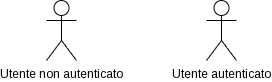
\includegraphics[width=0.6\columnwidth]{img/usecase/attori.png} 
    \caption{Gerarchia degli attori.}
    \label{fig:attori}
\end{figure}


\subsubsection{Elenco dei casi d'uso}

Segue l'elenco dei casi d'uso ritrovati, l'elenco è diviso essenzialmente in tre aree:
\begin{itemize}
    \item casi d'uso per l'autenticazione (figura \ref{fig:uc-auth});
    \item casi d'uso per la mappa dell'itinerario (figura \ref{fig:uc-map});
    \item casi d'uso per la visualizzazione in dettaglio dell'itinerario (figura \ref{fig:uc-tour}).
\end{itemize}

\noindent I casi d'uso di autenticazione si rivolgono alle azioni di autenicazione, di registrazione e di recupero password, i casi d'uso per la mappa dell'itinerario descrivono le azioni di condivisione della posizione e visualizzazione della mappa. Infine i casi d'uso per la visualizzazione in dettaglio dell'itinerario specificano le azioni di visualizzazione sulle componenti di un itinerario, quali: le giornate, le \textit{route}, i \textit{climb} e altre informazioni minori.

%%% GESTIONE AUTENTICAZIONE
\begin{figure}[!h] 
    \centering 
    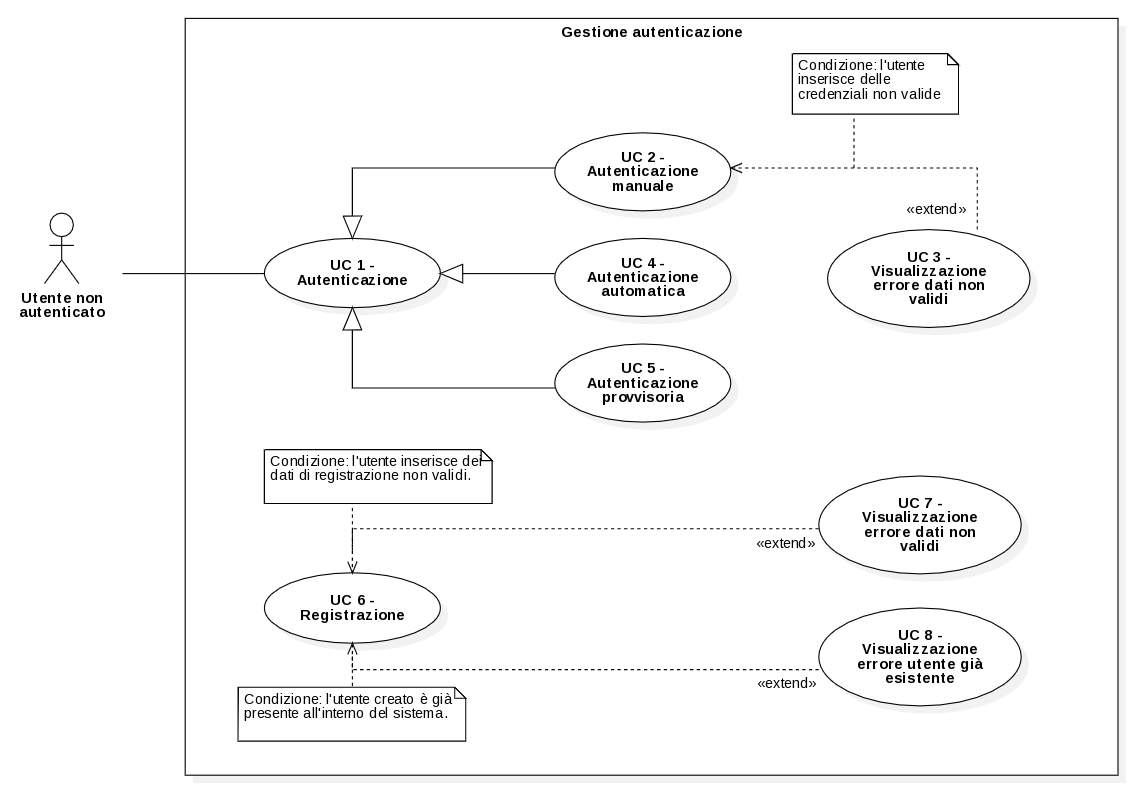
\includegraphics[width=0.9\columnwidth]{img/usecase/gestione-auth.png} 
    \caption{Casi d'uso relativi all'autenticazione.}
    \label{fig:uc-auth}
\end{figure}

\uc{Autenticazione}\label{uc:login}
\begin{itemize}
    \item \textbf{Attore primario}: utente non autenticato;
    \item \textbf{Descrizione}: l'utente deve potersi autenticare e accedere al proprio account;
    \item \textbf{Scenario principale}:
    \begin{enumerate}
        \item l'utente apre l'applicazione;
        \item l'utente si autentica normalmente (\textbf{\ref{uc:login_manuale}}), in modo automatico (\textbf{\ref{uc:login_automatico}}), se aveva precedentemente memorizzato la sessione, o accede con l'autenticazione provvisoria (\textbf{\ref{uc:login_prv}}).
    \end{enumerate}
    \item \textbf{Precondizioni}: l'utente non è ancora autenticato nel sistema;
    \item \textbf{Postcondizioni}: l'utente si è autenticato nel sistema.
\end{itemize}

\subuc{Autenticazione manuale}\label{uc:login_manuale}
\begin{itemize}
    \item \textbf{Attore}: utente non autenticato;
    \item \textbf{Descrizione}: l'utente deve potersi autenticare e accedere manualmente al proprio account;
    \item \textbf{Scenario principale}:
    \begin{enumerate}
        \item l'utente apre l'applicazione;
        \item l'utente inserisce la propria \textit{e-mail} (\textbf{\ref{uc:login_email}});
        \item l'utente inserisce la propria password (\textbf{\ref{uc:login_password}});
        \item se l'utente vuole, seleziona la casella di memorizzazione della sessione (\textbf{\ref{uc:login_ricordami}});
        \item l'utente conferma i dati inseriti (\textbf{\ref{uc:login_conferma}}).
    \end{enumerate}
    \item \textbf{Precondizioni}: l'utente non è ancora autenticato nel sistema;
    \item \textbf{Postcondizioni}:
    \begin{itemize}
        \item l'utente si è autenticato nel sistema;
        \item se l'utente ha selezionato la casella di memorizzazione della sessione, al prossimo accesso al sito verrà autenticato automaticamente.
    \end{itemize}
    \item \textbf{Estensioni}: l'utente inserisce delle credenziali non valide e viene mostrato un messaggio d'errore (\textbf{\ref{uc:login_err}}).
\end{itemize}
\begin{figure}[!h] 
    \centering 
    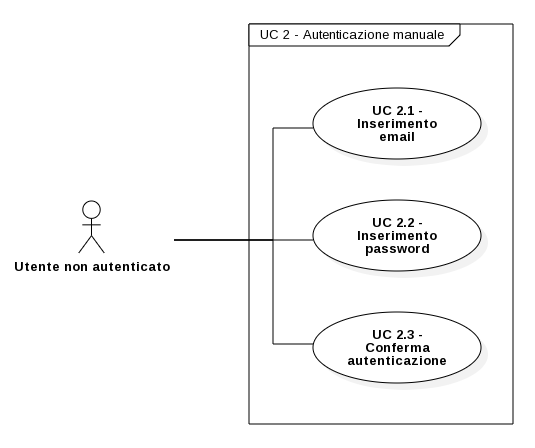
\includegraphics[width=0.9\columnwidth]{img/usecase/login-manuale.png} 
    \caption{Sottocasi d'uso di UC 2.}
\end{figure}

\subsubuc{Inserimento email}\label{uc:login_email}
\begin{itemize}
    \item \textbf{Attore primario}: utente non autenticato;
    \item \textbf{Descrizione}: l'utente deve poter inserire la propria \textit{e-mail} durante l'attività di autenticazione manuale;
    \item \textbf{Scenario principale}:
    \begin{enumerate}
        \item l'utente seleziona il campo relativo al nome utente;
        \item l'utente digita il proprio nome utente.
    \end{enumerate}
    \item \textbf{Precondizioni}: l'utente sta svolgendo l'attività di autenticazione;
    \item \textbf{Postcondizioni}: l'utente ha compilato il campo relativo al nome utente.
\end{itemize}

\subsubuc{Inserimento password}\label{uc:login_password}
\begin{itemize}
    \item \textbf{Attore primario}: utente non autenticato;
    \item \textbf{Descrizione}: l'utente deve poter inserire la propria password durante l'attività di autenticazione;
    \item \textbf{Scenario principale}:
    \begin{enumerate}
        \item l'utente seleziona il campo relativo alla password;
        \item l'utente digita la propria password.
    \end{enumerate}
    \item \textbf{Precondizioni}: l'utente sta svolgendo l'attività di autenticazione;
    \item \textbf{Postcondizioni}: l'utente ha compilato il campo relativo alla password.
\end{itemize}

\subuc{Conferma autenticazione}\label{uc:login_conferma}
\begin{itemize}
    \item \textbf{Attore primario}: utente non autenticato;
    \item \textbf{Descrizione}: l'utente deve poter confermare i dati inseriti e tentare di autenticarsi;
    \item \textbf{Scenario principale}: l'utente conferma l'azione di autenticazione;
    \item \textbf{Precondizioni}: l'utente sta svolgendo l'attività di autenticazione;
    \item \textbf{Postcondizioni}: l'utente ha tentato di autenticarsi utilizzando i dati inseriti.
\end{itemize}

\subuc{Autenticazione automatica}\label{uc:login_automatico}
\begin{itemize}
    \item \textbf{Attore primario}: utente non autenticato;
    \item \textbf{Descrizione}: l'utente deve poter essere autenticato automaticamente se ha memorizzato una sessione;
    \item \textbf{Scenario principale}:
    \begin{enumerate}
        \item l'utente accede al sito;
        \item l'utente viene automaticamente autenticato.
    \end{enumerate}
    \item \textbf{Precondizioni}: l'utente ha una sessione valida memorizzata;
    \item \textbf{Postcondizioni}: l'utente è autenticato.
\end{itemize}

\subuc{Memorizzazione sessione}\label{uc:login_ricordami}
\begin{itemize}
    \item \textbf{Attore primario}: utente non autenticato;
    \item \textbf{Descrizione}: l'utente deve poter richiedere la memorizzazione della sessione per effettuare automaticamente il autenticazione al prossimo accesso al sito;
    \item \textbf{Scenario principale}: l'utente seleziona la casella di memorizzazione della sessione;
    \item \textbf{Precondizioni}: l'utente sta svolgendo l'attività di autenticazione;
    \item \textbf{Postcondizioni}: l'utente ha richiesto la memorizzazione della sessione.
\end{itemize}

\uc{Autenticazione provvisoria}\label{uc:login_prv}
\begin{itemize}
    \item \textbf{Attore primario}: utente non autenticato;
    \item \textbf{Descrizione}: l'utente deve potersi autenticare e accedere a un account preesistente;
    \item \textbf{Scenario principale}:
    \begin{enumerate}
        \item l'utente apre l'applicazione;
        \item l'utente seleziona un utente preesistente (\textbf{\ref{uc:sel_user}});
        \item l'utente si autentica con l'utente selezionato (\textbf{\ref{uc:login_prov_conferma}}).
    \end{enumerate}
    \item \textbf{Precondizioni}: l'utente non è ancora autenticato nel sistema;
    \item \textbf{Postcondizioni}: l'utente si è autenticato nel sistema.
\end{itemize}
\begin{figure}[!h] 
    \centering 
    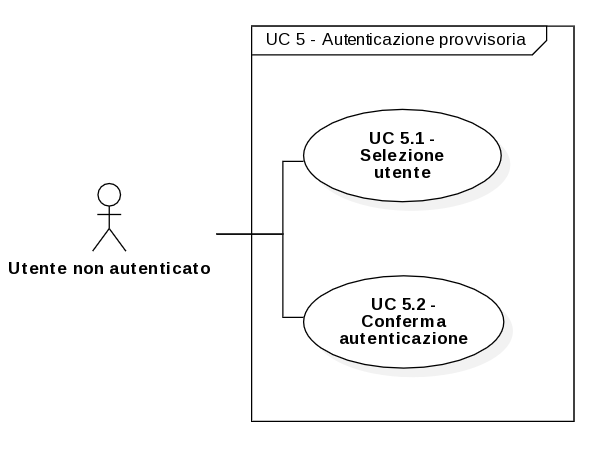
\includegraphics[width=0.9\columnwidth]{img/usecase/login-provvisorio.png} 
    \caption{Sottocasi d'uso di UC 5.}
\end{figure}

\subuc{Selezione utente}\label{uc:sel_user}
\begin{itemize}
    \item \textbf{Attore primario}: utente non autenticato;
    \item \textbf{Descrizione}: l'utente deve poter selezionare un utente preesistente nel sistema;
    \item \textbf{Scenario principale}: l'utente seleziona un utente preesistente nel sistema;
    \item \textbf{Precondizioni}: l'utente sta svolgendo l'attività di autenticazione provvisoria;
    \item \textbf{Postcondizioni}: l'utente ha compilato il campo relativo alla password.
\end{itemize}

\subuc{Conferma autenticazione}\label{uc:login_prov_conferma}
\begin{itemize}
    \item \textbf{Attore primario}: utente non autenticato;
    \item \textbf{Descrizione}: l'utente deve poter confermare i dati inseriti e tentare di autenticarsi;
    \item \textbf{Scenario principale}: l'utente conferma l'azione di autenticazione;
    \item \textbf{Precondizioni}: l'utente sta svolgendo l'attività di autenticazione;
    \item \textbf{Postcondizioni}: l'utente ha tentato di autenticarsi utilizzando i dati inseriti.
\end{itemize}

\uc{Visualizzazione errore dati inseriti non validi}\label{uc:login_err}
\begin{itemize}
    \item \textbf{Attore primario}: utente non autenticato;
    \item \textbf{Descrizione}: l'utente deve ricevere un errore a seguito dell'inserimento di credenziali non valide durante l'attività di autenticazione manuale;
    \item \textbf{Scenario principale}: l'utente visualizza un messaggio di errore;
    \item \textbf{Precondizioni}: l'utente sta svolgendo l'attività di autenticazione manuale e inserisce delle credenziali non valide;
    \item \textbf{Postcondizioni}: l'utente ha ricevuto un messaggio d'errore.
\end{itemize}

\uc{Registrazione}\label{uc:registrazione}
\begin{itemize}
    \item \textbf{Attore primario}: utente non autenticato;
    \item \textbf{Descrizione}: l'utente deve potersi registrare all'interno del sistema;
    \item \textbf{Precondizioni}: l'utente non è ancora autenticato nel sistema;
    \item \textbf{Scenario principale}:
    \begin{enumerate}
        \item l'utente apre l'applicazione;
        \item l'utente clicca il pulsante di registrazione (\textbf{\ref{uc:signup_nome}});
        \item l'utente inserisce il suo nome (\textbf{\ref{uc:signup_cognome}});
        \item l'utente inserisce il suo cognome (\textbf{\ref{uc:signup_mail}});
        \item l'utente inserisce la sua password (\textbf{\ref{uc:signup_pw}});
        \item l'utente inserisce nuovamente la password inserita in precedenza (\textbf{\ref{uc:signup_conferma_pw}});
        \item l'utente conferma i dati inseriti (\textbf{\ref{uc:signup_conferma}}).
    \end{enumerate}
    \item \textbf{Postcondizioni}: l'utente è registrato e autenticato nel sistema;
    \item \textbf{Estensioni}: 
    \begin{enumerate}
        \item l'utente inserisce dei dati non validi e viene mostrato un messaggio d'errore (\textbf{\ref{uc:reg_err_dati}});
        \item l'utente creato è già presente all'interno del sistema e viene mostrato un messaggio d'errore (\textbf{\ref{uc:reg_err_utente}}).
    \end{enumerate}
\end{itemize}
\begin{figure}[!h] 
    \centering 
    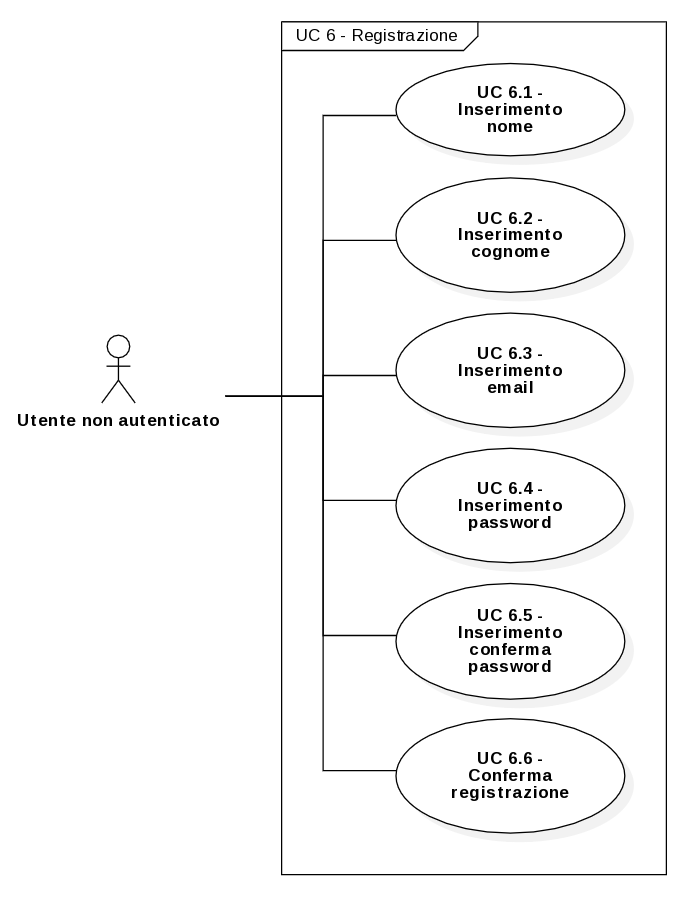
\includegraphics[width=0.9\columnwidth]{img/usecase/registrazione.png} 
    \caption{Sottocasi d'uso di UC 6.}
\end{figure}

\subuc{Inserimento nome}\label{uc:signup_nome}
\begin{itemize}
    \item \textbf{Attore primario}: utente non autenticato;
    \item \textbf{Descrizione}: l'utente deve poter inserire il proprio nome durante l'attività di registrazione;
    \item \textbf{Precondizioni}: l'utente sta svolgendo l'attività di registrazione;
    \item \textbf{Scenario principale}:
    \begin{enumerate}
        \item l'utente seleziona il campo relativo al nome;
        \item l'utente digita il proprio nome.
    \end{enumerate}
    \item \textbf{Postcondizioni}: l'utente ha compilato il campo relativo al nome.
\end{itemize}

\subuc{Inserimento cognome}\label{uc:signup_cognome}
\begin{itemize}
    \item \textbf{Attore primario}: utente non autenticato;
    \item \textbf{Descrizione}: l'utente deve poter inserire il proprio cognome durante l'attività di registrazione;
    \item \textbf{Scenario principale}:
    \begin{enumerate}
        \item l'utente seleziona il campo relativo al cognome;
        \item l'utente digita il proprio cognome.
    \end{enumerate}
    \item \textbf{Precondizioni}: l'utente sta svolgendo l'attività di registrazione;
    \item \textbf{Postcondizioni}: l'utente ha compilato il campo relativo al cognome.
\end{itemize}

\subuc{Inserimento email}\label{uc:signup_mail}
\begin{itemize}
    \item \textbf{Attore primario}: utente non autenticato;
    \item \textbf{Descrizione}: l'utente deve poter inserire la propria \textit{e-mail} durante l'attività di registrazione;
    \item \textbf{Precondizioni}: l'utente sta svolgendo l'attività di registrazione;
    \item \textbf{Scenario principale}:
    \begin{enumerate}
        \item l'utente seleziona il campo relativo all'\textit{email};
        \item l'utente digita la propria \textit{email}.
    \end{enumerate}
    \item \textbf{Postcondizioni}: l'utente ha compilato il campo relativo alla \textit{email}.
\end{itemize}

\subuc{Inserimento password}\label{uc:signup_pw}
\begin{itemize}
    \item \textbf{Attore primario}: utente non autenticato;
    \item \textbf{Descrizione}: l'utente deve poter inserire la propria password durante l'attività di autenticazione;
    \item \textbf{Precondizioni}: l'utente sta svolgendo l'attività di autenticazione;
    \item \textbf{Scenario principale}:
    \begin{enumerate}
        \item l'utente seleziona il campo relativo alla password;
        \item l'utente digita la propria password.
    \end{enumerate}
    \item \textbf{Postcondizioni}: l'utente ha compilato il campo relativo alla password.
\end{itemize}

\subuc{Inserimento conferma password}\label{uc:signup_conferma_pw}
\begin{itemize}
    \item \textbf{Attore primario}: utente non autenticato;
    \item \textbf{Descrizione}: l'utente deve poter inserire nuovamente la propria password durante l'attività di registrazione;
    \item \textbf{Precondizioni}: l'utente sta svolgendo l'attività di registrazione;
    \item \textbf{Scenario principale}:
    \begin{enumerate}
        \item l'utente seleziona il campo relativo alla conferma della password;
        \item l'utente digita nuovamente la propria password.
    \end{enumerate}
    \item \textbf{Postcondizioni}: l'utente ha compilato il campo relativo alla conferma della password.
\end{itemize}

\subuc{Conferma registrazione}\label{uc:signup_conferma}
\begin{itemize}
	\item \textbf{Attore primario}: utente non autenticato;
	\item \textbf{Descrizione}: l'utente conferma i dati inseriti relativi alla registrazione;
	\item \textbf{Precondizioni}: l'utente sta svolgendo l'attività di registrazione;
	\item \textbf{Scenario principale}: l'utente conferma i dati inseriti;
	\item \textbf{Postcondizioni}: l'utente viene creato nel sistema.
\end{itemize}

\uc{Visualizzazione errore dati inseriti non validi}\label{uc:reg_err_dati}
\begin{itemize}
    \item \textbf{Attore primario}: utente non autenticato;
    \item \textbf{Descrizione}: l'utente deve ricevere un errore a seguito dell'inserimento di credenziali non valide durante l'attività di registrazione;
    \item \textbf{Precondizioni}: l'utente sta svolgendo l'attività di registrazione e inserisce delle credenziali non valide;
    \item \textbf{Scenario principale}: l'utente visualizza un messaggio di errore;
    \item \textbf{Postcondizioni}: l'utente ha ricevuto un messaggio d'errore.
\end{itemize}

\uc{Visualizzazione errore utente già esistente}\label{uc:reg_err_utente}
\begin{itemize}
    \item \textbf{Attore primario}: utente non autenticato;
    \item \textbf{Descrizione}: l'utente deve ricevere un errore per aver tentato di creare un utente già presente nel sistema;
    \item \textbf{Precondizioni}: l'utente sta svolgendo l'attività di registrazione;
    \item \textbf{Scenario principale}: l'utente tenta di aggiungere un utente già presente nel sistema;
    \item \textbf{Postcondizioni}: l'utente ha ricevuto un messaggio d'errore.
\end{itemize}

%%% GESTIONE MAPPA
\begin{figure}[!h] 
    \centering 
    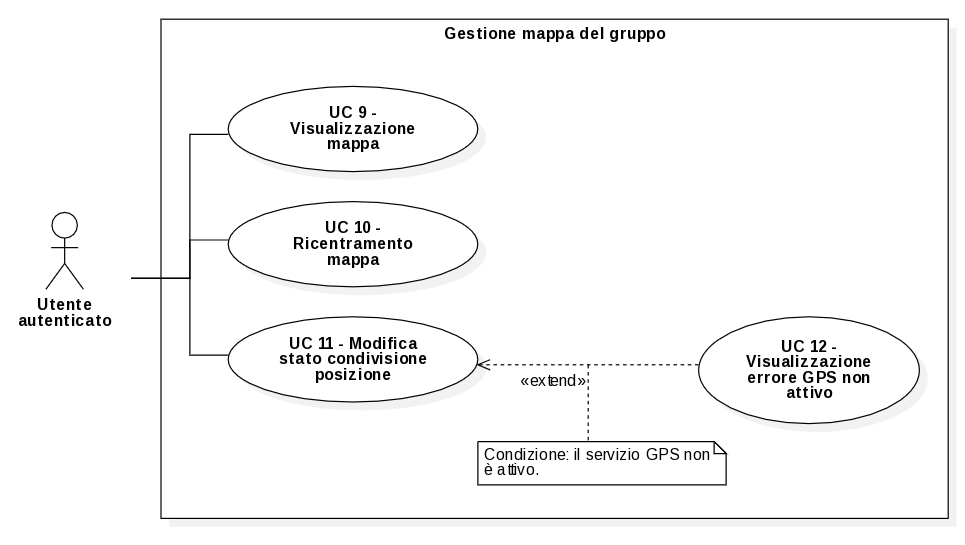
\includegraphics[width=0.9\columnwidth]{img/usecase/gestione-mappa.png} 
    \caption{Casi d'uso relativi alla gestione della mappa del gruppo.}
    \label{fig:uc-map}
\end{figure}

\uc{Visualizzazione mappa}\label{uc:vis_map}
\begin{itemize}
	\item \textbf{Attore primario}: utente autenticato;
	\item \textbf{Descrizione}: l'utente deve poter visualizzare tutti i partecipanti e il loro nome nella mappa, evidenziando l'utente stesso e il pulmino di soccorso;
    \item \textbf{Precondizioni}: l'utente si trova nella schermata di condivisione della posizione;
	\item \textbf{Scenario principale}:
    \begin{enumerate}
        \item l'utente visualizza tutti i partecipanti nella mappa, con il loro nome, distinguendo sè stesso e il pulmino di soccorso (\textbf{\ref{uc:view_group}});
        \item l'utente clicca su un partecipante e visualizza la distanza da esso (\textbf{\ref{uc:group_distance}}).
    \end{enumerate}
	\item \textbf{Postcondizioni}: l'utente visualizza la mappa del gruppo.
\end{itemize}

\subuc{Visualizzazione partecipanti}\label{uc:view_group}
\begin{itemize}
	\item \textbf{Attore primario}: utente autenticato;
	\item \textbf{Descrizione}: l'utente deve poter visualizzare i partecipanti nella mappa;
	\item \textbf{Precondizioni}: l'utente sta svolgendo l'attività di visualizzazione della mappa;
	\item \textbf{Scenario principale}: l'utente visualizza i partecipanti dell'itinerario nella mappa;
	\item \textbf{Postcondizioni}: l'utente sta svolgendo l'attività di visualizzazione della mappa.
\end{itemize}

\subuc{Visualizzazione distanze}\label{uc:group_distance}
\begin{itemize}
	\item \textbf{Attore primario}: utente autenticato;
	\item \textbf{Descrizione}: l'utente deve poter visualizzare la distanza tra lui e un altro partecipante;
	\item \textbf{Precondizioni}: l'utente sta svolgendo l'attività di visualizzazione della mappa;
	\item \textbf{Scenario principale}: l'utente clicca su un partecipante nella mappa;
	\item \textbf{Postcondizioni}: l'utente visualizza la distanza tra lui e il partecipante indicato.
\end{itemize}

\uc{Ricentramento mappa}\label{uc:recenter_map}
\begin{itemize}
	\item \textbf{Attore primario}: utente autenticato;
	\item \textbf{Descrizione}: l'utente deve poter ricentrare la mappa nella posizione in cui si trova;
	\item \textbf{Precondizioni}: l'utente non è centrato nella mappa;
	\item \textbf{Scenario principale}: l'utente clicca il pulsante di ricentramento della posizione;
	\item \textbf{Postcondizioni}: l'utente è centrato nella mappa.
\end{itemize}

\uc{Modifica stato condivisione posizione}\label{uc:modifica_stato_condivisione_posizione}
\begin{itemize}
	\item \textbf{Attore primario}: utente autenticato;
	\item \textbf{Descrizione}: l'utente deve poter condividere la sua posizione con il resto del gruppo;
	\item \textbf{Precondizioni}: l'utente si trova nella schermata di condivisione della posizione;
	\item \textbf{Scenario principale}: l'utente attiva (\textbf{\ref{uc:att_pos}}) o disattiva (\textbf{\ref{uc:dis_pos}}) la condivisione della posizione;
	\item \textbf{Postcondizioni}: l'utente condivide la sua posizione con il resto del gruppo;
    \item \textbf{Estensioni}: l'utente non ha il servizio GPS attivo e viene mostrato un messaggio d'errore (\textbf{\ref{uc:gps_err}}).
\end{itemize}
\begin{figure}[!h] 
    \centering 
    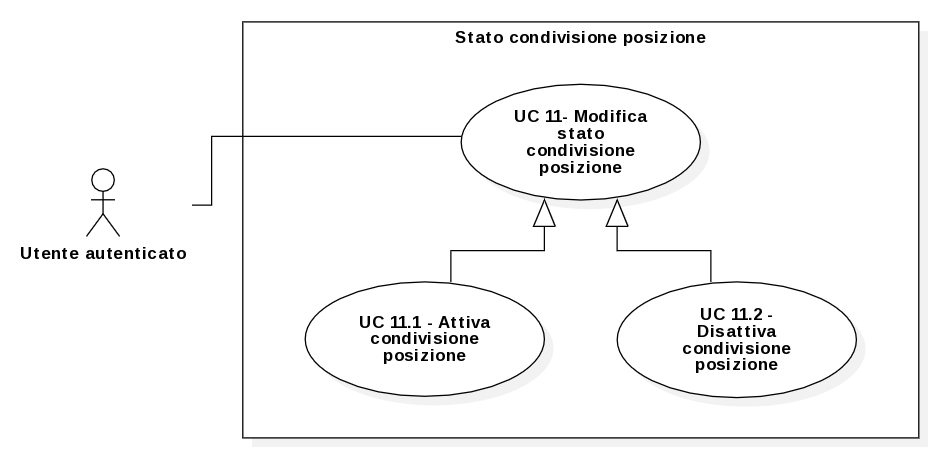
\includegraphics[width=0.9\columnwidth]{img/usecase/stato-condivisione.png} 
    \caption{Sottocasi d'uso di UC 11.}
\end{figure}

\subuc{Attiva condivisione posizione}\label{uc:att_pos}
\begin{itemize}
	\item \textbf{Attore primario}: utente autenticato;
	\item \textbf{Descrizione}: l'utente deve poter attivare la condivisione della posizione;
	\item \textbf{Precondizioni}: 
	\begin{enumerate}
		\item l'utente sta svolgendo l'attività di modifica dello stato di condivisione posizione;
		\item la condivisione della posizione è disattivata.
	\end{enumerate}
    \item \textbf{Scenario principale}: l'utente attiva la condivisione della posizione;
	\item \textbf{Postcondizioni}: la condivisione della posizione è attivata.
\end{itemize}

\subuc{Disattiva condivisione posizione}\label{uc:dis_pos}
\begin{itemize}
	\item \textbf{Attore primario}: utente autenticato;
	\item \textbf{Descrizione}: l'utente deve poter disattivare la condivisione della posizione;
	\item \textbf{Precondizioni}: 
	\begin{enumerate}
		\item l'utente sta svolgendo l'attività di modifica dello stato di condivisione posizione;
		\item la condivisione della posizione è attivata.
	\end{enumerate}
    \item \textbf{Scenario principale}: l'utente disattiva la condivisione della posizione;
	\item \textbf{Postcondizioni}: la condivisione della posizione è disattivata.
\end{itemize}

\uc{Visualizzazione errore GPS non attivo}\label{uc:gps_err}
\begin{itemize}
    \item \textbf{Attore primario}: utente autenticato;
    \item \textbf{Descrizione}: l'utente deve ricevere un errore a seguito dell'attivazione della condivisione della posizione nel caso in cui il GPS non sia attivato;
    \item \textbf{Precondizioni}: l'utente sta svolgendo l'attività di modifica stato condivisione posizione;
    \item \textbf{Scenario principale}: l'utente visualizza un messaggio di errore;
    \item \textbf{Postcondizioni}: l'utente ha ricevuto un messaggio d'errore.
\end{itemize}

\uc{Visualizzazione giornate itinerario}\label{uc:vis_it}
\begin{itemize}
	\item \textbf{Attore primario}: utente autenticato;
	\item \textbf{Descrizione}: l'utente deve poter visualizzare l'itinerario corrente;
	\item \textbf{Precondizioni}: l'utente si trova nella schermata degli itinerari;
	\item \textbf{Scenario principale}: l'utente visualizza tutte le giornate dell'itinerario corrente;
	\item \textbf{Postcondizioni}: l'utente visualizza l'itinerario corrente.
\end{itemize}

%%% GESTIONE GIORNATA ITINERARIO
\begin{figure}[!h] 
    \centering 
    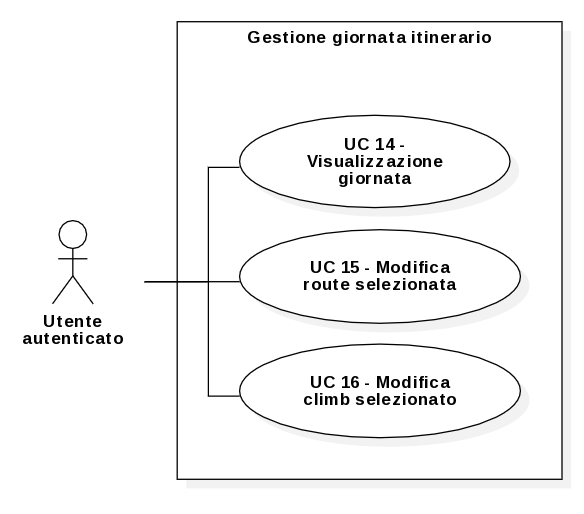
\includegraphics[width=0.9\columnwidth]{img/usecase/gestione-giornata.png} 
    \caption{Casi d'uso relativi alla gestione dell'itinerario.}
    \label{fig:uc-tour}
\end{figure}

\uc{Visualizzazione giornata}\label{uc:vis_day}
\begin{itemize}
	\item \textbf{Attore primario}: utente autenticato;
	\item \textbf{Descrizione}: l'utente deve poter visualizzare una giornata di un itinerario in dettaglio;
    \item \textbf{Precondizioni}: l'utente si trova nella schermata degli itinerari;
	\item \textbf{Scenario principale}:
    \begin{enumerate}
        \item l'utente visualizza la mappa della giornata (\textbf{\ref{uc:vis_mappa}});
        \item l'utente visualizza un \textit{POI} in dettaglio (\textbf{\ref{uc:vis_poi}});
        \item l'utente visualizza un \textit{climb} in dettaglio (\textbf{\ref{uc:vis_climb}}).
    \end{enumerate}
	\item \textbf{Postcondizioni}: l'utente visualizza una giornata in dettaglio.
\end{itemize}
\begin{figure}[!h] 
    \centering 
    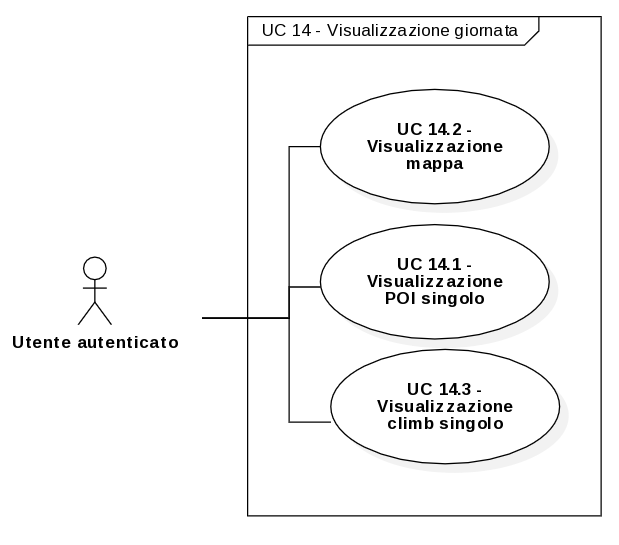
\includegraphics[width=0.9\columnwidth]{img/usecase/vis-day.png} 
    \caption{Sottocasi d'uso di UC 14.}
\end{figure}

\subuc{Visualizzazione mappa}\label{uc:vis_mappa}
\begin{itemize}
	\item \textbf{Attore primario}: utente autenticato;
	\item \textbf{Descrizione}: l'utente deve poter visualizzare la mappa della giornata;
    \item \textbf{Precondizioni}: l'utente si trova nella schermata degli itinerari;
	\item \textbf{Scenario principale}:
    \begin{enumerate}
        \item l'utente visualizza i partecipanti (\textbf{\ref{uc:vis_partecipanti}});
        \item l'utente visualizza tutti i POI (\textbf{\ref{uc:vis_poi_map_day}});
        \item l'utente visualizza il \textit{climb} al momento selezionato (\textbf{\ref{uc:vis_climb_sel}});
        \item l'utente visualizza la \textit{route} al momento selezionata (\textbf{\ref{uc:vis_route_sel}});
        \item l'utente visualizza la route percorsa dai partecipanti (\textbf{\ref{uc:vis_route_percorsa}}).
    \end{enumerate}
	\item \textbf{Postcondizioni}: l'utente visualizza la mappa di una giornata.
\end{itemize}
\begin{figure}[!h] 
    \centering 
    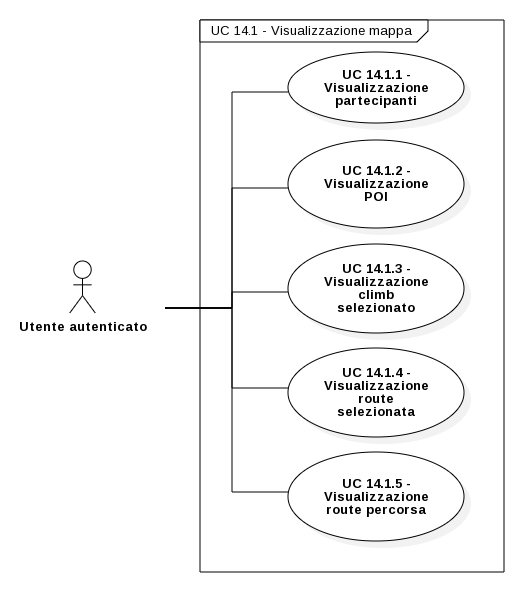
\includegraphics[width=0.9\columnwidth]{img/usecase/vis-map.png} 
    \caption{Sottocasi d'uso di UC 14.1.}
\end{figure}

\subsubuc{Visualizzazione partecipanti}\label{uc:vis_partecipanti}
\begin{itemize}
	\item \textbf{Attore primario}: utente autenticato;
	\item \textbf{Descrizione}: l'utente deve poter visualizzare i partecipanti nella mappa;
	\item \textbf{Precondizioni}: l'utente sta svolgendo l'attività di visualizzazione della mappa;
	\item \textbf{Scenario principale}: l'utente visualizza i partecipanti dell'itinerario nella mappa;
	\item \textbf{Postcondizioni}: l'utente sta svolgendo l'attività di visualizzazione della mappa.
\end{itemize}

\subsubuc{Visualizzazione POI}\label{uc:vis_poi_map_day}
\begin{itemize}
	\item \textbf{Attore primario}: utente autenticato;
	\item \textbf{Descrizione}: l'utente deve poter visualizzare i \textit{POI} nella mappa;
	\item \textbf{Precondizioni}: l'utente sta svolgendo l'attività di visualizzazione della mappa;
	\item \textbf{Scenario principale}: l'utente visualizza tutti i \textit{POI} dell'itinerario nella mappa;
	\item \textbf{Postcondizioni}: l'utente sta svolgendo l'attività di visualizzazione della mappa.
\end{itemize}

\subsubuc{Visualizzazione \textit{climb} selezionato}\label{uc:vis_climb_sel}
\begin{itemize}
	\item \textbf{Attore primario}: utente autenticato;
	\item \textbf{Descrizione}: l'utente deve poter visualizzare il \textit{climb} selezionato nella mappa;
	\item \textbf{Precondizioni}: l'utente sta svolgendo l'attività di visualizzazione della mappa;
	\item \textbf{Scenario principale}: l'utente visualizza il \textit{climb} selezionato nella mappa;
	\item \textbf{Postcondizioni}: l'utente sta svolgendo l'attività di visualizzazione della mappa.
\end{itemize}

\subsubuc{Visualizzazione \textit{route} selezionata}\label{uc:vis_route_sel}
\begin{itemize}
	\item \textbf{Attore primario}: utente autenticato;
	\item \textbf{Descrizione}: l'utente deve poter visualizzare la \textit{route} selezionata nella mappa;
	\item \textbf{Precondizioni}: l'utente sta svolgendo l'attività di visualizzazione della mappa;
	\item \textbf{Scenario principale}: l'utente visualizza la \textit{route} selezionata nella mappa;
	\item \textbf{Postcondizioni}: l'utente sta svolgendo l'attività di visualizzazione della mappa.
\end{itemize}

\subsubuc{Visualizzazione \textit{route} percorsa}\label{uc:vis_route_percorsa}
\begin{itemize}
	\item \textbf{Attore primario}: utente autenticato;
	\item \textbf{Descrizione}: l'utente deve poter visualizzare la \textit{route} percorsa da un partecipante;
	\item \textbf{Precondizioni}: l'utente sta svolgendo l'attività di visualizzazione mappa;
	\item \textbf{Scenario principale}: l'utente clicca su un partecipante nella mappa;
	\item \textbf{Postcondizioni}: l'utente visualizza la \textit{route} percorsa.
\end{itemize}

\subuc{Visualizzazione POI singolo}\label{uc:vis_poi}
\begin{itemize}
	\item \textbf{Attore primario}: utente autenticato;
	\item \textbf{Descrizione}: l'utente deve poter visualizzare un \textit{POI} in dettaglio;
    \item \textbf{Precondizioni}: l'utente si trova nella schermata delle giornate;
	\item \textbf{Scenario principale}:
    \begin{enumerate}
        \item l'utente clicca su un \textit{POI};
        \item l'utente seleziona un \textit{POI} della giornata;
        \item l'utente visualizza il \textit{POI} selezionato nella mappa;
        \item l'utente visualizza le caratteristiche del \textit{POI} selezionato.
    \end{enumerate}
	\item \textbf{Postcondizioni}: l'utente si trova nella schermata dei poi.
\end{itemize}

\subuc{Visualizzazione climb singolo}\label{uc:vis_climb}
\begin{itemize}
	\item \textbf{Attore primario}: utente autenticato;
	\item \textbf{Descrizione}: l'utente deve poter visualizzare un \textit{climb} in dettaglio;
    \item \textbf{Precondizioni}: l'utente si trova nella schermata delle giornate;
	\item \textbf{Scenario principale}:
    \begin{enumerate}
        \item l'utente clicca su un poi;
        \item l'utente seleziona un \textit{climb} della giornata;
        \item l'utente visualizza il \textit{climb} selezionato nella mappa;
        \item l'utente visualizza le caratteristiche del \textit{climb} selezionato.
    \end{enumerate}
	\item \textbf{Postcondizioni}: l'utente si trova nella schermata dei climb.
\end{itemize}

\uc{Selezione route}\label{uc:sel_route}
\begin{itemize}
    \item \textbf{Attore primario}: utente non autenticato;
    \item \textbf{Descrizione}: l'utente deve poter selezionare una route di una giornata;
    \item \textbf{Precondizioni}: l'utente si trova nella schermata delle giornate;
    \item \textbf{Scenario principale}: l'utente seleziona una route di una giornata;
    \item \textbf{Postcondizioni}: l'utente selezionato una route.
\end{itemize}

\uc{Selezione climb}\label{uc:sel_climb}
\begin{itemize}
    \item \textbf{Attore primario}: utente non autenticato;
    \item \textbf{Descrizione}: l'utente deve poter selezionare un climb di una giornata;
    \item \textbf{Precondizioni}: l'utente si trova nella schermata delle giornate;
    \item \textbf{Scenario principale}: l'utente seleziona un climb di una giornata;
    \item \textbf{Postcondizioni}: l'utente selezionato un climb.
\end{itemize}

\subsection{Requisiti}
In questa sezione vengono elencati i requisiti individuati a seguito dell'analisi delle \gls{userstoryg}, dei casi d'uso, del dialogo con il cliente e la discussione con il \textit{project manager}. Un requisito può essere:
\begin{itemize}
    \item \textbf{funzionale}: se indica un vincolo sugli utilizzi e funzioni del prodotto;
    \item \textbf{di qualità}: se indica un vincolo imposto sulle tecniche o strumenti di sviluppo;
    \item \textbf{di vincolo}: se indica un vincolo imposto dall'azienda o dal cliente;
    \item \textbf{prestazionale}: se indica un vincolo da rispettare in determinate condizioni. 
\end{itemize}

\noindent Il codice di un requisito riflette il seguente formato:
\begin{center}
    \texttt{R[importanza][tipologia][numero]}
\end{center}
\noindent dove:
\begin{itemize}
    \item \texttt{[importanza]} è:
    \begin{itemize}
        \item \textbf{O}: per un requisito obbligatorio;
        \item \textbf{D}: per un requisito desiderabile;
        \item \textbf{P}: per un requisito opzionale.
    \end{itemize}
    \item \texttt{[tipologia]} è:
    \begin{itemize}
        \item \textbf{F}: per un requisito funzionale;
        \item \textbf{Q}: per un requisito di qualità;
        \item \textbf{V}: per un requisito di vincolo;
        \item \textbf{P}: per un requisito prestazionale.
    \end{itemize}
    \item \texttt{[numero]} è un numero progressivo univoco se il requisito non ha padre, altrimenti è nel formato: \begin{center} \texttt{[numero\_padre].[numero\_figlio]} \end{center} dove:
    \begin{itemize}
        \item \texttt{[numero\_padre]} è il \texttt{[numero]} del requisito padre;
        \item \texttt{[numero\_figlio]} è un numero progressivo univoco tra i figli dello stesso padre.
    \end{itemize}
\end{itemize}

\subsubsection{Requisiti funzionali}
\begin{longtable}{ |p{2cm}|p{8cm}|p{2cm}|  }
    \caption{Requisiti funzionali.}
    \label{tab:req-funzionali}
    \hline
    \textbf{Codice} & \textbf{Requisito} & \textbf{Fonte}
    \hline
    \textbf{ROF1}   & L'utente non autenticato deve potersi autenticare e accedere al proprio account & \textbf{UC 1}   \\ \hline
    \textbf{ROF2}   & L'utente non autenticato deve potersi autenticare manualmente. & \textbf{UC 2}   \\ \hline
    \textbf{ROF2.1} & L'utente non autenticato deve poter inserire la propria email durante l'attività di autenticazione manuale. & \textbf{UC 2.1} \\ \hline
    \textbf{ROF2.2} & L'utente non autenticato deve poter inserire la propria password durante l'attività du autenticazione manuale. & \textbf{UC 2.2} \\ \hline
    \textbf{ROF2.3} & L'utente non autenticato deve poter richiedere la memorizzazione della sessione durante l'attività di login. & \textbf{UC 2.3} \\ \hline
    \textbf{ROF2.4} & L'utente non autenticato deve poter confermare i dati inseriti e tentare di autenticarsi. & \textbf{UC 2.4} \\ \hline
    \textbf{ROF3}   & Il tentativo di autenticazione deve fallire nel caso in cui siano state inserite credenziali non valide. & \textbf{UC 3}   \\ \hline
    \textbf{ROF4}   & L'utente non autenticato deve potersi autenticare automaticamente nel caso in cui abbia memorizzato la sessione precedentemente. & \textbf{UC 4}   \\ \hline
    \textbf{ROF5}   & L'utente non autenticato deve potersi autenticare in modo provvisorio. & \textbf{UC 5} \\ \hline
    \textbf{ROF5.1} & L'utente non autenticato deve poter selezionare un utente preesistente durante l'attività di autenticazione provvisoria & \textbf{UC 5.1} \\ \hline
    \textbf{ROF5.2} & L'utente non autenticato deve poter confermare l'utente preesistente selezionato e tentare di autenticarsi. & \textbf{UC 5.2} \\ \hline
    \textbf{ROF6}   & L'utente non autenticato deve potersi registrare. & \textbf{UC 6} \\ \hline
    \textbf{ROF6.1} & L'utente non autenticato deve poter inserire il proprio nome durante l'attività di registrazione. & \textbf{UC 6.1} \\ \hline
    \textbf{ROF6.2} & L'utente non autenticato deve poter inserire il proprio cognome durante l'attività di registrazione. & \textbf{UC 6.2} \\ \hline
    \textbf{ROF6.3} & L'utente non autenticato deve poter inserire la propria email durante l'attività di registrazione. & \textbf{UC 6.3} \\ \hline
    \textbf{ROF6.4} & L'utente non autenticato deve poter inserire la propria password durante l'attività di registrazione. & \textbf{UC 6.4} \\ \hline
    \textbf{ROF6.5} & L'utente non autenticato deve poter confermare la propria password durante l'attività di registrazione. & \textbf{UC 6.5} \\ \hline
    \textbf{ROF6.6} & L'utente non autenticato deve poter confermare i dati inseriti e tentare di registrarsi. & \textbf{UC 6.6} \\ \hline
    \textbf{ROF7}   & Il tentativo di registrazione deve fallire nel caso in cui siano stati inseriti dati di registrazione non validi. & \textbf{UC 7}   \\ \hline
    \textbf{ROF8}   & Il tentativo di registrazione deve fallire nel caso in cui l'utente creato sia già presente nel sistema. & \textbf{UC 8}   \\ \hline
    \textbf{ROF9}   & L'utente autenticato deve poter visualizzare la mappa dell'itinerario. & \textbf{UC 9}   \\ \hline
    \textbf{ROF9.1} & L'utente autenticato deve poter visualizzare la sua distanza con gli altri partecipanti. & \textbf{UC 9.1} \\ \hline
    \textbf{ROF9.2} & L'utente autenticato deve poter visualizzare l'accuratezza del suo segnale \textit{GPS}. & \textbf{UC 9.2} \\ \hline
    \textbf{ROF10}  & L'utente autenticato deve poter ricentrare la mappa nella sua posizione. & \textbf{UC 10}  \\ \hline
    \textbf{ROF11}  & L'utente autenticato deve modificare lo stato di condivisione della propria posizione. & \textbf{UC 11}  \\ \hline
    \textbf{ROF11.1} & L'utente autenticato deve poter attivare la condivisione della posizione. & \textbf{UC 11.1} \\ \hline
    \textbf{ROF11.2} & l'utente autenticato deve poter disattivare la condivisione della posizione. & \textbf{UC 11.2} \\ \hline
    \textbf{ROF12} & Il tentativo di attivazione della condivisione della posizione deve fallire nel caso in cui il GPS non sia attivo. & \textbf{UC 12} \\ \hline
    \textbf{ROF13} & L'utente autenticato deve poter visualizzare tutte le giornate dell'itinerario corrente. & \textbf{UC 13} \\ \hline
    \textbf{ROF14} & L'utente autenticato deve poter visualizzare una giornata nel dettaglio. & \textbf{UC 14} \\ \hline
    \textbf{ROF14.1} & L'utente autenticato deve poter visualizzare la mappa durante l'attività di visualizzazione di una giornata nel dettaglio. & \textbf{UC 14.1} \\ \hline
    \textbf{ROF14.1.1} & L'utente autenticato deve poter visualizzare i partecipanti durante l'attività di visualizzazione della mappa di una giornata. & \textbf{UC 14.1.1}\\ \hline
    \textbf{ROF14.1.2} & L'utente autenticato deve poter visualizzare tutti i \textit{POI} durante l'attività di visualizzazione della mappa di una giornata. & \textbf{UC 14.1.2}\\ \hline
    \textbf{ROF14.1.3} & L'utente autenticato deve poter visualizzare la \textit{route} percorsa di un partecipante durante l'attività di visualizzazione della mappa di una giornata. & \textbf{UC 14.1.3}\\ \hline
    \textbf{ROF14.1.4} & L'utente autenticato deve poter visualizzare la \textit{route} selezionata durante l'attività di visualizzazione della mappa di una giornata. & \textbf{UC 14.1.4} \\ \hline
    \textbf{ROF14.1.5} & L'utente autenticato deve poter visualizzare il \textit{climb} selezionato durante l'attività di visualizzazione della mappa di una giornata. & \textbf{UC 14.1.5} \\ \hline
    \textbf{ROF14.1.6} & I \textit{POI} generici e speciali devono essere visualizzati differentemente nella mappa di una giornata. & \textbf{UC 14.1.6} \\ \hline
    \textbf{ROF14.2} & L'utente autenticato deve poter visualizzare i \textit{climb} di una giornata durante l'attività di visualizzazione di una giornata nel dettaglio. & \textbf{UC 14.2} \\ \hline
    \textbf{ROF14.3} & L'utente autenticato deve poter visualizzare i \textit{poi} di una giornata durante l'attività di visualizzazione di una giornata nel dettaglio. & \textbf{UC 14.3} \\ \hline
    \textbf{ROF15} & L'utente autenticato deve poter modificare la \textit{route} selezionata in una giornata. & \textbf{UC 15} \\ \hline
    \textbf{ROF16} & L'utente autenticato deve poter modificare il \textit{climb} selezionato in una giornata. & \textbf{UC 16} \\ \hline
\end{longtable}

\subsubsection{Requisiti di qualità}
\begin{longtable}{ |p{2cm}|p{8cm}|p{2cm}|  }
    \caption{Requisiti di qualità.}
    \label{tab:req-qualita}
    \hline
    \textbf{Codice} & \textbf{Requisito} & \textbf{Fonte}
    \hline
    \textbf{ROQ1} & L'applicazione deve essere sviluppata con in \textit{dart}. & \textbf{Azienda} \\ \hline
    \textbf{ROQ2} & L'applicazione deve essere sviluppata con il \textit{framework} \textit{flutter}. & \textbf{Azienda} \\ \hline
    \textbf{RDQ2.1} & l'applicazione \textit{flutter} deve essere sviluppata con il \textit{bloc pattern}. & \textbf{Azienda} \\ \hline
    \textbf{ROQ3} & I sorgenti devono essere versionati con lo strumento \textit{git}. & \textbf{Azienda} \\ \hline
    \textbf{ROQ4} & Il repository remoto per il versionamento destinato all'azienda deve essere \textit{BitBucket}. & \textbf{Azienda} \\ \hline
    \textbf{ROQ5} & Il repository remoto per il versionamento destinato al cliente deve essere \textit{GitHub}. & \textbf{Cliente} \\ \hline
    \textbf{ROQ6} & Il \textit{back-end} dell'applicazione deve esporre un \textit{API} \gls{restg}. & \textbf{Cliente} \\ \hline
    \textbf{RDQ7} & La base di dati per il salvataggio in locale dei dati deve essere \textit{Sqlite}.  & \textbf{Cliente} \\ \hline
\end{longtable}


\subsubsection{Requisiti di vincolo}
\begin{longtable}{ |p{2cm}|p{8cm}|p{2cm}|  }
    \caption{Requisiti di vincolo.}
    \label{tab:req-vincolo}
    \hline
    \textbf{Codice} & \textbf{Requisito} & \textbf{Fonte}
    \hline
    \textbf{ROV1} & La posizione dell'utente dell'applicazione deve essere riconoscibile. & \textbf{Cliente} \\ \hline
    \textbf{ROV2} & La posizione del pulmino di soccorso deve essere riconoscibile. & \textbf{Cliente} \\ \hline
    \textbf{ROV3} & La giornata corrente di un itinerario deve essere evidenziata. & \textbf{Cliente} \\ \hline
    \textbf{RDV4} & Se l'utente ha ricentrato la sua posizione, la mappa deve ricentrarsi automaticamente nel caso in cui l'utente aggiorni la sua posizione. & \textbf{Azienda} \\ \hline
    \textbf{RDV5} & Il tratto di \textit{route} percorsa deve essere visualizzata nella mappa. & \textbf{Azienda} \\ \hline
    \textbf{ROV6} & I \textit{POI} normali devono essere visulizzati differentemente da quelli speciali. & \textbf{Cliente} \\ \hline
    \textbf{ROV7} & L'interfaccia dell'applicazione deve seguire il più fedelmente possibile i \textit{mockup} dell'applicazione. & \textbf{Cliente} \\ \hline
    \textbf{ROV8} & La condivisione della posizione deve poter funzionare anche in \textit{background}. & \textbf{Cliente}\\ \hline
\end{longtable}

\subsubsection{Requisiti prestazionali}
\begin{longtable}{ |p{2cm}|p{8cm}|p{2cm}|  }
    \caption{Requisiti prestazionali.}
    \label{tab:req-prestazioni}
    \hline
    \multicolumn{3}{|c|}{Tabella dei requisiti}
    \hline
    \textbf{Codice} & \textbf{Requisito} & \textbf{Fonte} \\ \hline
    \textbf{ROP1} & L'invio della propria posizione deve avvenire solo quando l'utente si muove di almento cinque metri & \textbf{Azienda} \\ \hline
    \textbf{ROP2} & La ricezione delle posizioni del gruppo deve avvenire ogni trenta secondi & \textbf{Cliente} \\ \hline
    \textbf{RDP3} & I \textit{GPX} non devono essere richiesti più di una volta & \textbf{Azienda} \\ \hline
\end{longtable} 


\subsection{Tracciamento}
\subsubsection{Fonte - Requisiti}
\begin{longtable}{ |p{3cm}|p{3cm}|  }
    \caption{Tracciamento fonte - requisiti.}
    \label{tab:req-tracciamento}
    \hline
    \textbf{Fonte} & \textbf{Requisito}
    \hline
    \textbf{Azienda} &
                 \textbf{ROQ1}
        \newline \textbf{ROQ2}
        \newline \textbf{RDQ2.1}
        \newline \textbf{ROQ3}
        \newline \textbf{ROQ4}
        \newline \textbf{ROQ5}
        \newline \textbf{ROQ6}
        \newline \textbf{RDQ7}
        \newline \textbf{RDV4}
        \newline \textbf{RDV5}
        \newline \textbf{ROP1}
        \newline \textbf{RDP3}
        \hline
    \textbf{Cliente} &
                 \textbf{ROQ5} 
        \newline \textbf{ROQ6} 
        \newline \textbf{RDQ7} 
        \newline \textbf{ROV1}
        \newline \textbf{ROV2}
        \newline \textbf{ROV3}
        \newline \textbf{ROV6}
        \newline \textbf{ROV7}
        \newline \textbf{ROV8}
        \newline \textbf{ROP2}
        \hline
    \textbf{UC 1}       & \textbf{ROF1}        \\ \hline
    \textbf{UC 2}       & \textbf{ROF2}        \\ \hline
    \textbf{UC 2.1}     & \textbf{ROF2.1}      \\ \hline
    \textbf{UC 2.2}     & \textbf{ROF2.2}      \\ \hline
    \textbf{UC 2.3}     & \textbf{ROF2.3}      \\ \hline
    \textbf{UC 2.4}     & \textbf{ROF2.4}      \\ \hline
    \textbf{UC 3}       & \textbf{ROF3}        \\ \hline
    \textbf{UC 4}       & \textbf{ROF4}        \\ \hline
    \textbf{UC 5}       & \textbf{ROF5}        \\ \hline
    \textbf{UC 5.1}     & \textbf{ROF5.1}      \\ \hline
    \textbf{UC 5.2}     & \textbf{ROF5.2}      \\ \hline
    \textbf{UC 6}       & \textbf{ROF6}        \\ \hline
    \textbf{UC 6.1}     & \textbf{ROF6.1}      \\ \hline
    \textbf{UC 6.2}     & \textbf{ROF6.2}      \\ \hline
    \textbf{UC 6.3}     & \textbf{ROF6.3}      \\ \hline
    \textbf{UC 6.4}     & \textbf{ROF6.4}      \\ \hline
    \textbf{UC 6.5}     & \textbf{ROF6.5}      \\ \hline
    \textbf{UC 6.6}     & \textbf{ROF6.6}      \\ \hline
    \textbf{UC 7}       & \textbf{ROF7}        \\ \hline
    \textbf{UC 8}       & \textbf{ROF8}        \\ \hline
    \textbf{UC 9}       & \textbf{ROF9}        \\ \hline
    \textbf{UC 9.1}     & \textbf{ROF9.1}      \\ \hline
    \textbf{UC 9.2}     & \textbf{ROF9.2}      \\ \hline
    \textbf{UC 10}      & \textbf{ROF10}       \\ \hline
    \textbf{UC 11}      & \textbf{ROF11}       \\ \hline
    \textbf{UC 11.1}    & \textbf{ROF11.1}     \\ \hline
    \textbf{UC 11.2}    & \textbf{ROF11.2}     \\ \hline
    \textbf{UC 12}      & \textbf{ROF12}       \\ \hline
    \textbf{UC 13}      & \textbf{ROF13}       \\ \hline
    \textbf{UC 14}      & \textbf{ROF14}       \\ \hline
    \textbf{UC 14.1}    & \textbf{ROF14.1}     \\ \hline
    \textbf{UC 14.1.1}  & \textbf{ROF14.1.1}   \\ \hline
    \textbf{UC 14.1.2}  & \textbf{ROF14.1.2}   \\ \hline
    \textbf{UC 14.1.3}  & \textbf{ROF14.1.3}   \\ \hline
    \textbf{UC 14.1.4}  & \textbf{ROF14.1.4}   \\ \hline
    \textbf{UC 14.1.5}  & \textbf{ROF14.1.5}   \\ \hline
    \textbf{UC 14.1.6}  & \textbf{ROF14.1.6}   \\ \hline
    \textbf{UC 14.2}    & \textbf{ROF14.2}     \\ \hline
    \textbf{UC 14.3}    & \textbf{ROF14.3}     \\ \hline
    \textbf{UC 15}      & \textbf{ROF15}       \\ \hline
    \textbf{UC 16}      & \textbf{ROF16}       \\ \hline
\end{longtable}

\subsubsection{Requisiti - Fonte}
\begin{longtable}{ |p{3cm}|p{3cm}|  }
    \caption{Tracciamento requisiti - fonte.}
    \label{tab:req-tracciamento-inverso}
    \hline
    \textbf{Requisito} & \textbf{Fonte}
    \hline
    \textbf{ROF1}   &   \textbf{UC 1}   \\ \hline
    \textbf{ROF2}   &   \textbf{UC 2}   \\ \hline
    \textbf{ROF2.1} &   \textbf{UC 2.1} \\ \hline
    \textbf{ROF2.2} &   \textbf{UC 2.2} \\ \hline
    \textbf{ROF2.3} &   \textbf{UC 2.3} \\ \hline
    \textbf{ROF2.4} &   \textbf{UC 2.4} \\ \hline
    \textbf{ROF3}   &   \textbf{UC 3}   \\ \hline
    \textbf{ROF4}   &   \textbf{UC 4}   \\ \hline
    \textbf{ROF5}   &   \textbf{UC 5}   \\ \hline
    \textbf{ROF5.1} &   \textbf{UC 5.1} \\ \hline
    \textbf{ROF5.2} &   \textbf{UC 5.2} \\ \hline
    \textbf{ROF6}   &   \textbf{UC 6}   \\ \hline
    \textbf{ROF6.1} &   \textbf{UC 6.1} \\ \hline
    \textbf{ROF6.2} &   \textbf{UC 6.2} \\ \hline
    \textbf{ROF6.3} &   \textbf{UC 6.3} \\ \hline
    \textbf{ROF6.4} &   \textbf{UC 6.4} \\ \hline
    \textbf{ROF6.5} &   \textbf{UC 6.5} \\ \hline
    \textbf{ROF6.6} &   \textbf{UC 6.6} \\ \hline
    \textbf{ROF7}   &   \textbf{UC 7}   \\ \hline
    \textbf{ROF8}   &   \textbf{UC 8}   \\ \hline
    \textbf{ROF9}   &   \textbf{UC 9}   \\ \hline
    \textbf{ROF9.1} &   \textbf{UC 9.1} \\ \hline
    \textbf{ROF9.2} &   \textbf{UC 9.2} \\ \hline
    \textbf{ROF10}  &   \textbf{UC 10}  \\ \hline
    \textbf{ROF11}  &   \textbf{UC 11}  \\ \hline
    \textbf{ROF11.1} &  \textbf{UC 11.1} \\ \hline
    \textbf{ROF11.2} &  \textbf{UC 11.2} \\ \hline
    \textbf{ROF12} &    \textbf{UC 12} \\ \hline
    \textbf{ROF13} &    \textbf{UC 13} \\ \hline
    \textbf{ROF14} &    \textbf{UC 14} \\ \hline
    \textbf{ROF14.1} &  \textbf{UC 14.1} \\ \hline
    \textbf{ROF14.1.1} & \textbf{UC 14.1.1}\\ \hline
    \textbf{ROF14.1.2} & \textbf{UC 14.1.2}\\ \hline
    \textbf{ROF14.1.3} & \textbf{UC 14.1.3}\\ \hline
    \textbf{ROF14.1.4} & \textbf{UC 14.1.4} \\ \hline
    \textbf{ROF14.1.5} & \textbf{UC 14.1.5} \\ \hline
    \textbf{ROF14.1.6} & \textbf{UC 14.1.6} \\ \hline
    \textbf{ROF14.2} &   \textbf{UC 14.2} \\ \hline
    \textbf{ROF14.3} &   \textbf{UC 14.3} \\ \hline
    \textbf{ROF15} &     \textbf{UC 15} \\ \hline
    \textbf{ROF16} &     \textbf{UC 16} \\ \hline
    \textbf{ROQ1} &      \textbf{Azienda} \\ \hline
    \textbf{ROQ2} &      \textbf{Azienda} \\ \hline
    \textbf{RDQ2.1} &    \textbf{Azienda} \\ \hline
    \textbf{ROQ3} & \textbf{Azienda} \\ \hline
    \textbf{ROQ4} & \textbf{Azienda} \\ \hline
    \textbf{ROQ5} & \textbf{Cliente} \\ \hline
    \textbf{ROQ6} & \textbf{Cliente} \\ \hline
    \textbf{RDQ7} & \textbf{Cliente} \\ \hline
    \textbf{ROP1} & \textbf{Cliente} \\ \hline
    \textbf{ROP2} & \textbf{Cliente} \\ \hline
    \textbf{ROP3} & \textbf{Cliente} \\ \hline
    \textbf{RDF4} & \textbf{Azienda} \\ \hline
    \textbf{RDF5} & \textbf{Azienda} \\ \hline
    \textbf{ROF6} & \textbf{Cliente} \\ \hline
    \textbf{ROF7} & \textbf{Cliente} \\ \hline
    \textbf{ROF8} & \textbf{Cliente}\\ \hline
    \textbf{ROP1} & \textbf{Azienda} \\ \hline
    \textbf{ROP2} & \textbf{Cliente} \\ \hline
    \textbf{RDP3} & \textbf{Azienda} \\ \hline
\end{longtable}


\subsubsection{Riepilogo}

La tabella \ref{tab:req-riepilogo} presenta il riepilogo dei requisiti.
\begin{longtable}{|c|c|c|c|c|}
        \caption{Riepilogo dei requisiti.}
        \label{tab:req-riepilogo}
        \hline
        \textbf{Tipologia} & \textbf{Obbligatori} & \textbf{Opzionali} & \textbf{Desiderabili} & \textbf{Totale}
        \hline
        Funzionali & 40 & 0 & 0 & 40 \\ \hline
        Di qualità & 6 & 0 & 2 & 8 \\ \hline
        Di vincolo & 6 & 0 & 2 & 8 \\ \hline
        Prestazionali & 2 & 0 & 1 & 3 \\ \hline
        \textbf{Totale} & 54 & 0 & 5 & 59 \hline
\end{longtable}

\newpage
\section{Progettazione}

\subsection{Architettura di sistema}

L'architettura segue un normale \textit{modello client-server}, nella quale l'applicazione flutter svolge il ruolo di client e il \textit{back-end} offerto dal cliente svolge quello di server. Tralasciando l'architettura del \textit{back-end}, andiamo ad analizzare l'archittura dell'applicazione da me sviuluppata. 

\subsubsection{Architettura dell'applicazione}

L'architettura dell'applicazione è illustrata nella figura \ref{fig:architettura}, questa si basa in larga parte al modello presentato in §\ref{lb:cenni-bloc}. Sono presenti due package principali, \textit{Presentation} e \textit{Data}, il primo si occupa di tutto ciò che concerne l'interazione con l'utente, quindi la visualizzaione delle schermate e gli eventi, il secondo si occupa di tutto ciò che concerne i dati di dominio dell'applicazione, fornendo punti di accesso e operazioni su di essi. Il terzo package \textit{Utils} si occupa solo di mantenere delle classi ausiliarie e non rappresenta un fattore architetturale di rilievo.

\begin{figure}[!h] 
    \centering 
    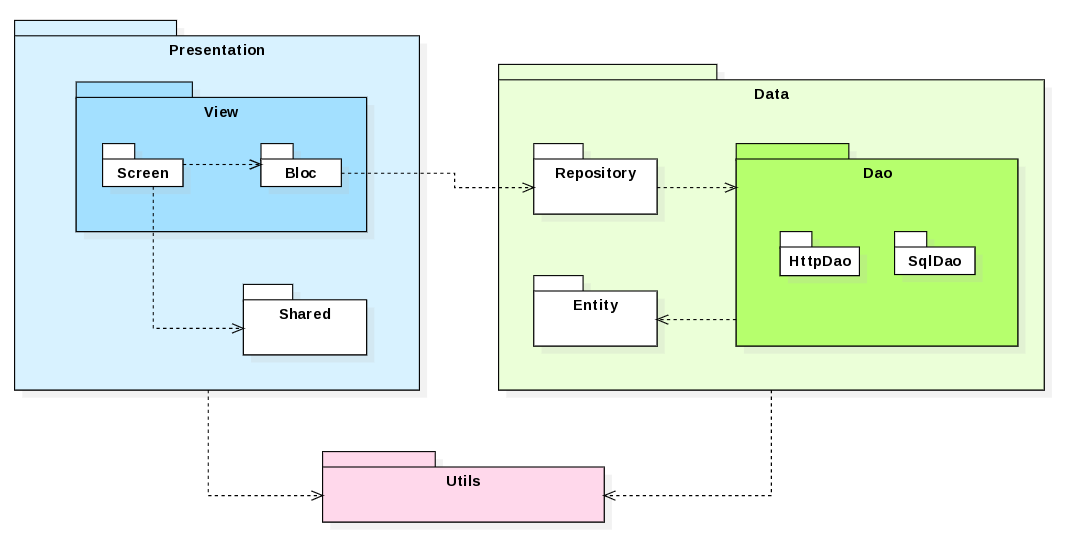
\includegraphics[width=0.9\columnwidth]{img/progettazione/architettura.png} 
    \caption{Architettura di CyclingHero.}
    \label{fig:architettura}
\end{figure}

\subsubsection{Descrizione delle componenti}

Dall'architettura di sistema si individuano le principali componenti, questa sezione si occupa di fornire una breve descrizione sulle loro funzioni.

\paragraph{Presentation}\\

Si occupa di costruire la parte grafica dell'applicazione e gestire l'interazione con l'utente, si compone di:
\begin{itemize}
    \item \textbf{View}: definisce le schermate dell'applicazione, si compone di:
        \begin{itemize}
            \item \textbf{Screen}: definisce una schermata in modo strutturale sulla base dello stato dal relativo \textit{bloc};
            \item \textbf{Bloc}: definisce gli aspetti comportamentali di una schermata, tramite eventi e stati, comunica direttamente con i \textit{repository}.
        \end{itemize}
    \item \textbf{Shared}: definisce gli elementi comuni per ogni schermata.
\end{itemize}

\paragraph{Data}\\

Si occupa di reperire e manipolare i dati dell'applicazione, si compone di;
\begin{itemize}
    \item \textbf{Repository}: definisce l'interfaccia di accesso ai dati, comunica direttamente con i \textit{Dao};
    \item \textbf{Dao}: fornisce l'implementazione per l'accesso ai dati in diverse sorgenti, nel caso dell'applicazione a quelle \gls{httpg} e \textit{SQL};
    \item \textbf{Entity}: definisce le entità partecipanti nel sistema.
\end{itemize}

\newpage
\section{Codifica}
In questa sezione vengono presentate le principali schermate dell'applicazione, per ogni schermata viene elaborata una descrizione sintetica e una lista di funzionalità implementate, successivamente viene analizzato in dettaglio il lato tecnico di tale interfaccia, accompagnando il tutto con dei diagrammi di sequenza per le attività rilevanti.

\subsection{Gestione dell'autenticazione}
In questa sezione vengono analizzate le schermate di autenticazione manuale e provvisoria, le altre schermate inerenti all'autenticazione, cioè quella di registrazione e recupero password sono analoghe a quella di autenticazione manuale, perciò non verranno approfondite.

\subsubsection{Descrizione}
\textit{CyclingHero} permette l'autenticazione per due differenti vie: quella manuale e quella provvisoria (figura \ref{fig:inter-auth}) .
La schermata di autenticazione manuale permette all'utente di collegarsi all'applicazione inserendo le sue credenziali, mentre quella provvisoria consente l'autenticazione tramite la scelta di un utente preesistente.
La schermata di autenticazione provvisoria è stata richiesta dal cliente in quanto \textit{back-end} non disponeva ancora di un \textit{API} per l'autenticazione. 
\newpage
\subsubsection{Interfaccia}
\begin{figure}[!h]
    \centering
    \frame{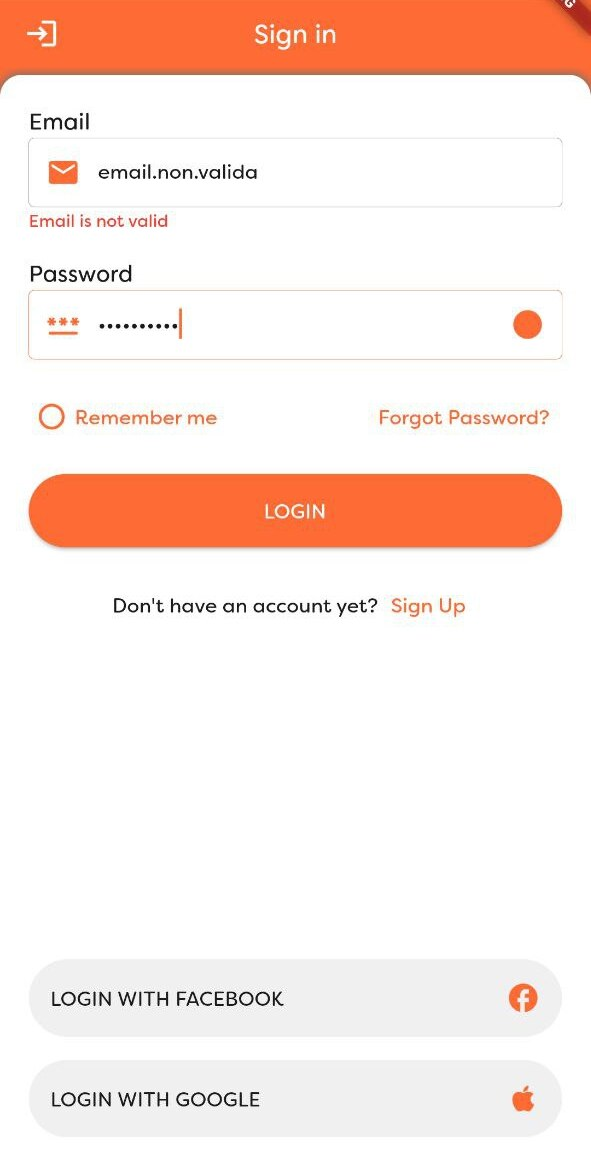
\includegraphics[width=0.4\columnwidth]{img/ch/login.jpg}}
    \frame{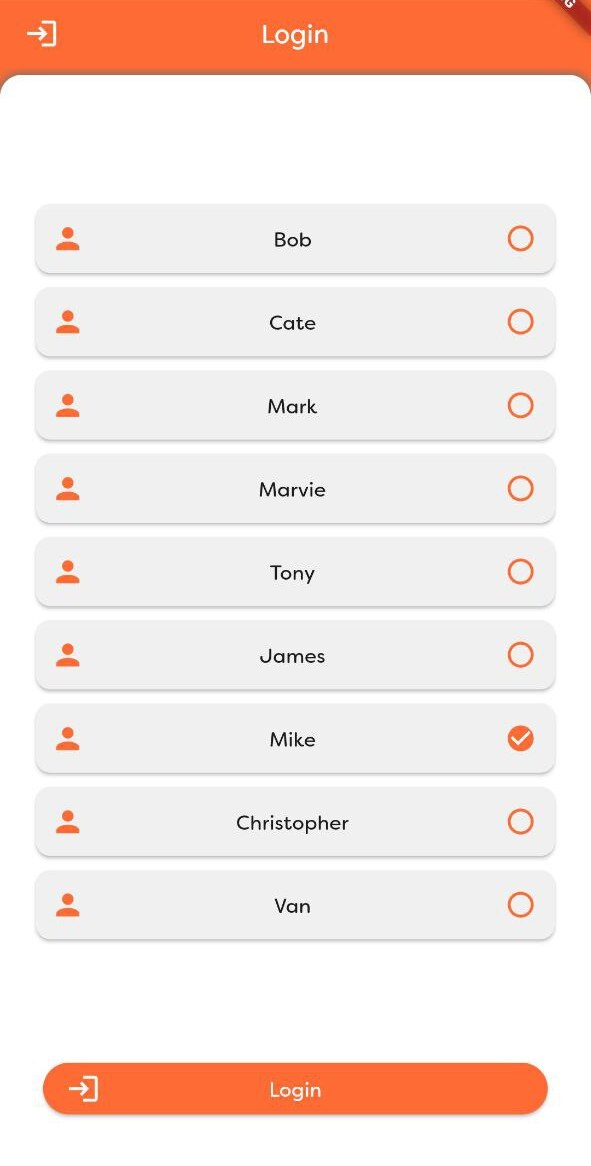
\includegraphics[width=0.4\columnwidth]{img/ch/legacy-login.jpg}}
    \caption{Da sinistra verso destra: schermata di autenticazione manuale, schermata di autenticazione provvisoria.}
    \label{fig:inter-auth}
\end{figure}

\subsubsection{Implementazione}
\paragraph{Schermata di autenticazione manuale}\\
La schermata di autenticazione manuale è basata fondamentalmente sulle seguenti classi:
\begin{itemize}
    \item \textbf{LoginScreen}: determina l'aspetto grafico della schermata, qui viene definita la gerarchia di \textit{widget} che compone la schermata. I principali \textit{widget} utilizzati sono: \textit{InputFieldCh} per l'acquisizione dei dati e\textit{ButtonCh} per i pulsanti di autenticazione;
    \item \textbf{LoginBloc}: rappresenta l'aspetto logico della schermata e svolge tre importanti compiti:
    \begin{itemize}
        \item definisce tutti gli eventi inerenti alla schermata, tra cui \textit{SubmitLoginEvent} per indicare l'azione di autenticazione e \textit{InputChangedEvent} per indicare la modifica di un campo del modulo;
        \item definisce lo stato della schermata, contiene gli \textit{InputField} e lo stato di autenticazione;
        \item gestisce gli eventi in arrivo interfacciandosi con lo strato sottostante con il \textit{UserRepository} per gestire l'autenticazione.
    \end{itemize}
    \item \textbf{InputField}: è una classe da me concepita per astrarre il concetto di campo di \textit{input}, questa classe svolge tre compiti:
    \begin{itemize}
        \item mantiene il valore dell'input rappresentato;
        \item mantiene lo stato di validazione dell'intput.
    \end{itemize}
\end{itemize}

\noindent  Nella figura \ref{fig:seq-auth} viene mostrato il diagramma di sequenza per processo di autenticazione. Per prima cosa l'evento \textit{SubmitLoginEvent} viene lanciato dalla schermata, \textit{LoginBloc}, dopo aver ricevuto l'evento e verificato la validità degli input, aggiorna il suo stato interno indicando un attesa di autenticazione che \textit{LoginScreen} interpreterà con la visualizzazione di un messaggio di attesa. Successivamente, \textit{LoginBloc} relega l'attività di autenticazione a \textit{UserRepository} che allo stesso modo incarica \textit{UserHttpDao} per finalizzare la richiesta all'\textit{API}. In caso di successo, \textit{UserRepository} si occuperà di gestire il contesto di autenticazione per l'applicazione e successivamente invierà a \textit{LoginBloc} l'esito dell'operazione, in quel momento \textit{LoginBloc} aggiornarà lo stato di successo di autenticazione, che si ripercuoterà nella schermata di autenticazione visualizzando un messaggio di successo.

\begin{figure}[!h]
    \centering
    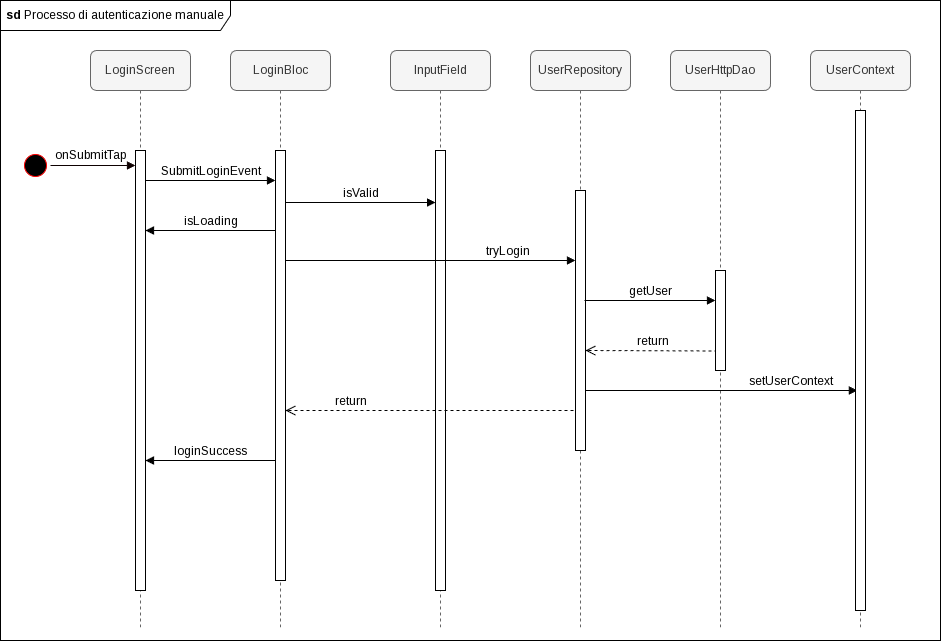
\includegraphics[width=0.9\columnwidth]{img/codifica/seq-auth.png}
    \caption{Diagramma di sequenza per il processo di autenticazione.}
    \label{fig:seq-auth}
\end{figure}


\paragraph{Schermata di autenticazione manuale}\\
La schermata di autenticazione provvisoria è stata un esigenza del cliente per ovviare la mancanza degli \textit{endpoint} di autenticazione. Come illustrato nel diagramma di sequenza della figura \ref{fig:seq-auth-prov}, l'autenticazione avviene semplicemente selezionando uno degli utenti preesistenti.

\begin{figure}[!h]
    \centering
    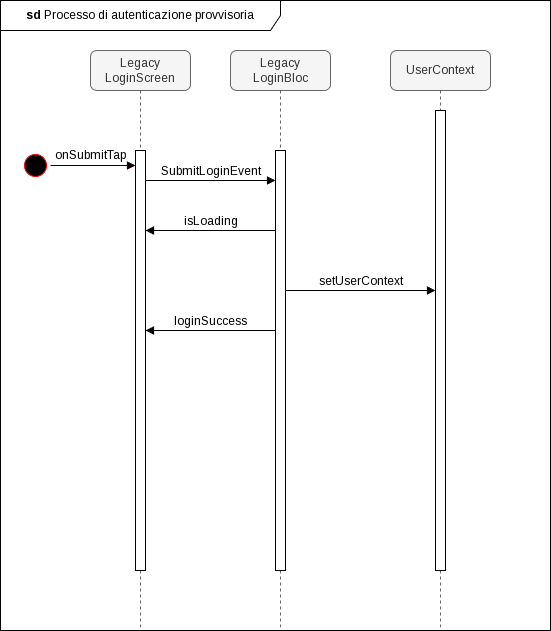
\includegraphics[width=0.7\columnwidth]{img/codifica/seq-legacy-auth.png}
    \caption{Diagramma di sequenza per il processo di autenticazione provvisoria.}
    \label{fig:seq-auth-prov}
\end{figure}

\subsubsection{Resoconto dei requisiti associati}
La tabella \ref{tab:req-auth-stato} elenca i requisiti associati all'attività di autenticazione. Sebbene nell'applicazione le funzionalità per l'autenticazione siano presenti, la mancanza del relativo \textit{endpoint} del \textit{back-end} non permette effettivamente l'autenticazione, perciò non sono riuscito a soddisfare tutti i requisiti di autenticazione.

\begin{longtable}{ |p{2cm}|p{8cm}|p{2cm}|  }
    \caption{Soddisfacimento dei requisiti associati alla gestione dell'autenticazione.}
    \label{tab:req-auth-stato}
    \hline
    \textbf{Codice} & \textbf{Descrizione} & \textbf{Stato}
    \hline
    \textbf{ROF1}   & L'utente non autenticato deve potersi autenticare e accedere al proprio account & \textbf{Soddisfatto}   \\ \hline
    \textbf{ROF2}   & L'utente non autenticato deve potersi autenticare manualmente. & \textbf{Non soddisfatto}   \\ \hline
    \textbf{ROF2.1} & L'utente non autenticato deve poter inserire la propria email durante l'attività di autenticazione manuale. & \textbf{Soddisfatto} \\ \hline
    \textbf{ROF2.2} & L'utente non autenticato deve poter inserire la propria password durante l'attività du autenticazione manuale. & \textbf{Soddisfatto} \\ \hline
    \textbf{ROF2.3} & L'utente non autenticato deve poter richiedere la memorizzazione della sessione durante l'attività di login. & \textbf{Soddisfatto} \\ \hline
    \textbf{ROF2.4} & L'utente non autenticato deve poter confermare i dati inseriti e tentare di autenticarsi. & \textbf{Non soddisfatto} \\ \hline
    \textbf{ROF3}   & Il tentativo di autenticazione deve fallire nel caso in cui siano state inserite credenziali non valide. & \textbf{Soddisfatto}   \\ \hline
    \textbf{ROF4}   & L'utente non autenticato deve potersi autenticare automaticamente nel caso in cui abbia memorizzato la sessione precedentemente. & \textbf{Non soddisfatto}   \\ \hline
    \textbf{ROF5}   & L'utente non autenticato deve potersi autenticare in modo provvisorio. & \textbf{Soddisfatto} \\ \hline
    \textbf{ROF5.1} & L'utente non autenticato deve poter selezionare un utente preesistente durante l'attività di autenticazione provvisoria & \textbf{Soddisfatto} \\ \hline
    \textbf{ROF5.2} & L'utente non autenticato deve poter confermare l'utente preesistente selezionato e tentare di autenticarsi. & \textbf{Soddisfatto} \\ \hline
    \textbf{ROF6}   & L'utente non autenticato deve potersi registrare. & \textbf{Non soddisfatto} \\ \hline
    \textbf{ROF6.1} & L'utente non autenticato deve poter inserire il proprio nome durante l'attività di registrazione. & \textbf{Soddisfatto} \\ \hline
    \textbf{ROF6.2} & L'utente non autenticato deve poter inserire il proprio cognome durante l'attività di registrazione. & \textbf{Soddisfatto} \\ \hline
    \textbf{ROF6.3} & L'utente non autenticato deve poter inserire la propria email durante l'attività di registrazione. & \textbf{Soddisfatto} \\ \hline
    \textbf{ROF6.4} & L'utente non autenticato deve poter inserire la propria password durante l'attività di registrazione. & \textbf{Soddisfatto} \\ \hline
    \textbf{ROF6.5} & L'utente non autenticato deve poter confermare la propria password durante l'attività di registrazione. & \textbf{Soddisfatto} \\ \hline
    \textbf{ROF6.6} & L'utente non autenticato deve poter confermare i dati inseriti e tentare di registrarsi. & \textbf{Non soddisfatto} \\ \hline
    \textbf{ROF7}   & Il tentativo di registrazione deve fallire nel caso in cui siano stati inseriti dati di registrazione non validi. & \textbf{Soddisfatto}   \\ \hline
    \textbf{ROF8}   & Il tentativo di registrazione deve fallire nel caso in cui l'utente creato sia già presente nel sistema. & \textbf{Non soddisfatto}   \\ \hline
\end{longtable}

\subsection{Gestione della mappa del gruppo}
\subsubsection{Descrizione}
La schermata di condivisione della posizioni (figura \ref{fig:inter-map}) consente all'utente di condividere e ricevere le posizioni del gruppo, offre inoltre un meccanismo per ricentrare la mappa in modo intelligente. Infine consente di visualizzare il gruppo e la propria distanza da ogni partecipante.

\newpage
\subsubsection{Interfaccia}
\begin{figure}[!h]
    \centering
    \frame{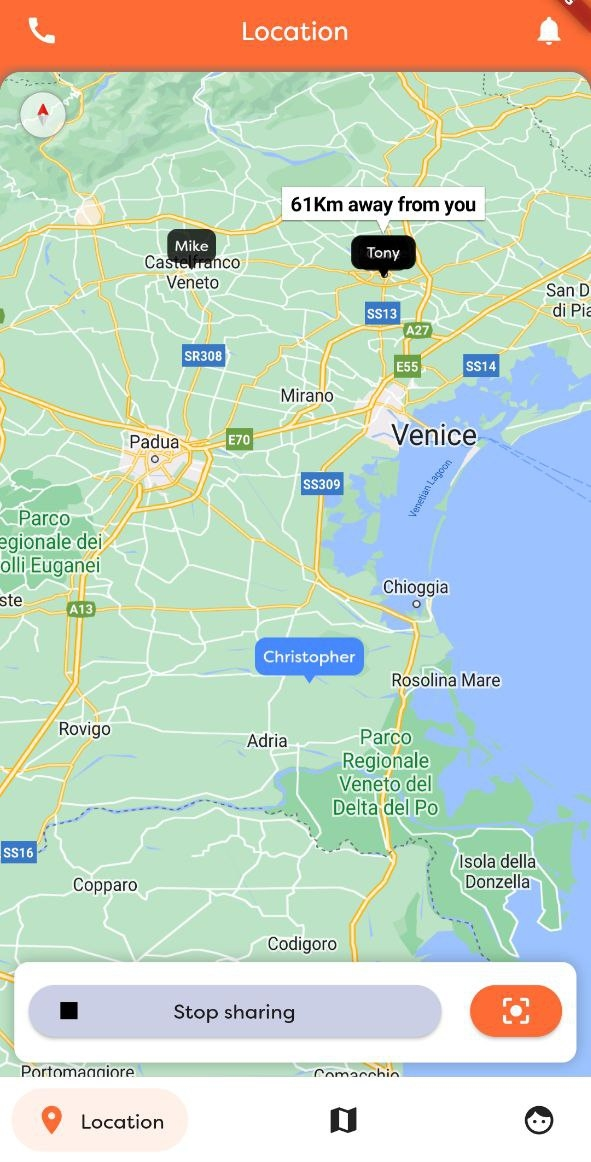
\includegraphics[width=0.4\columnwidth]{img/ch/location-sharing.jpg}}
    \caption{Schermata della mappa principale del gruppo.}
    \label{fig:inter-map}
\end{figure}

\subsubsection{Implementazione}
La schermata principale della mappa del gruppo è basata fondamentalmente sulle seguenti classi:
\begin{itemize}
    \item \textbf{LocationScreen}: determina l'aspetto grafico della schermata, qui viene definita la gerarchia di \textit{widget} che compone la schermata. I dati per la visualizzazione degli utenti sono contenuti nel \textit{LocationBloc}. I principali \textit{widget} utilizzati sono: \textit{GoogleMapCh} per visualizzare la mappa e disegnare gli utenti, \textit{ButtonCh} per i pulsanti di condivisione e ricentramento e \textit{PanelCh} per il pannello a scorrimento contenente le impostazioni di condivisione;
    \item \textbf{LocationBloc}: rappresenta l'aspetto logico della schermata e svolge tre importanti compiti:
    \begin{itemize}
        \item definisce tutti gli eventi inerenti alla schermata, tra cui \textit{ToggleSharingEvent} per attivare o disattivare la condivisione della posizione, \textit{LoadGroupEvent} per ricevere le posizioni degli altri partecipanti e \textit{CenterMapEvent} per centrare la mappa nella posizione dell'utente;
        \item definisce lo stato della schermata salvandosi le posizioni dei partecipanti;
        \item gestisce gli eventi in arrivo interfacciandosi con lo strato sottostante con il \textit{UserRepository} per gestire la ricezione e l'invio dei dati.
    \end{itemize}
    \item \textbf{LocationUtils}: è una classe da me concepita per semplificare l'\textit{API} di accesso alla posizione del dispositivo.
\end{itemize}

\begin{figure}[!h]
    \centering
    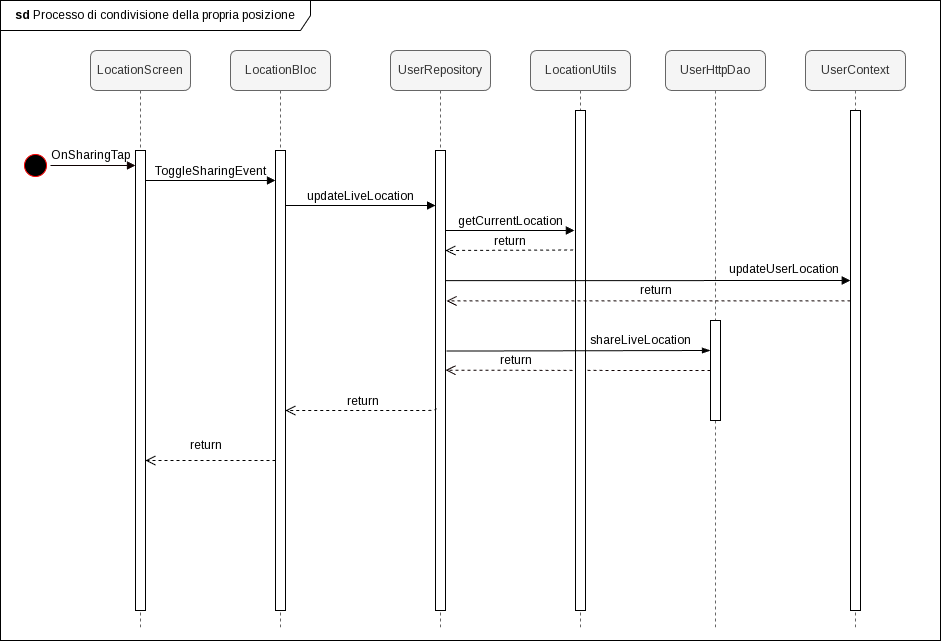
\includegraphics[width=0.9\columnwidth]{img/codifica/seq-share-loc.png}
    \caption{Diagramma di sequenza per il processo di condivisione della posizione.}
    \label{fig:seq-map}
\end{figure}

\noindent Il diagramma di sequenza in figura \ref{fig:seq-map} mostra il normale processo di condivisione della posizione: dopo aver ricevunto l'evento di attivazione della posizione, \textit{LocationBloc} invia una richiesta al \textit{userRepository} per avviare la condivisione. Per far questo \textit{UserRepository} inizia a rimanere in ascolto delle variazioni della posizione del dispositivo, se \textit{LocationUtils} rileva una variazione della posizione superiore di cinque metri rispetto alla precedente, allora informa il \textit{UserRepository} del nuovo dato, che passerà al \textit{UserHttpDao} per condivederla con il \textit{back-end}. Il processo nel suo complesso non è bloccnte per il \textit{LocationScreen}, che dopo il primo evento emesso in modo asincrono ritorna normalmente operativa.

\subsubsection{Resoconto dei requisiti associati}
La tabella \ref{tab:req-map-stato} elenca i requisiti associati all'attività di autenticazione. Ogni requisito identificato è stato soddisfatto e validato dal cliente.

\begin{longtable}{ |p{2cm}|p{8cm}|p{2cm}|  }
    \caption{Soddisfacimento dei requisiti associati alla gestione della mappa del gruppo.}
    \label{tab:req-map-stato}
    \hline
    \textbf{Codice} & \textbf{Descrizione} & \textbf{Stato}
    \hline
    \textbf{ROF9}   & L'utente autenticato deve poter visualizzare la mappa dell'itinerario. & \textbf{Soddisfatto}   \\ \hline
    \textbf{ROF9.1} & L'utente autenticato deve poter visualizzare la sua distanza con gli altri partecipanti. & \textbf{Soddisfatto} \\ \hline
    \textbf{ROF9.2} & L'utente autenticato deve poter visualizzare l'accuratezza del suo segnale \textit{GPS}. & \textbf{Soddisfatto} \\ \hline
    \textbf{ROF10}  & L'utente autenticato deve poter ricentrare la mappa nella sua posizione. & \textbf{Soddisfatto}  \\ \hline
    \textbf{ROF11}  & L'utente autenticato deve modificare lo stato di condivisione della propria posizione. & \textbf{Soddisfatto}  \\ \hline
    \textbf{ROF11.1} & L'utente autenticato deve poter attivare la condivisione della posizione. & \textbf{Soddisfatto} \\ \hline
    \textbf{ROF11.2} & L'utente autenticato deve poter disattivare la condivisione della posizione. & \textbf{Soddisfatto} \\ \hline
    \textbf{ROF12} & Il tentativo di attivazione della condivisione della posizione deve fallire nel caso in cui il GPS non sia attivo. & \textbf{Soddisfatto} \\ \hline
    \textbf{ROV1} & La posizione dell'utente dell'applicazione deve essere riconoscibile. & \textbf{Soddisfatto} \\ \hline
    \textbf{ROV2} & La posizione del pulmino di soccorso deve essere riconoscibile. & \textbf{Soddisfatto} \\ \hline
    \textbf{RDV4} & Se l'utente ha ricentrato la sua posizione, la mappa deve ricentrarsi automaticamente nel caso in cui l'utente aggiorni la sua posizione. & \textbf{Soddisfatto} \\ \hline
    \textbf{ROV8} & La condivisione della posizione deve poter funzionare anche in \textit{background}. & \textbf{Soddisfatto}\\ \hline
    \textbf{ROP1} & L'invio della propria posizione deve avvenire solo quando l'utente si muove di almento cinque metri & \textbf{Soddisfatto} \\ \hline
    \textbf{ROP2} & la ricezione delle posizioni del gruppo deve avvenire ogni trenta secondi & \textbf{Soddisfatto} \\ \hline
\end{longtable}


\subsection{Gestione dell'itinerario}
\subsubsection{Descrizione}
La gestione dell'itinerario (figura \ref{fig:inter-route}) è un processo implementato da più schermate:
\begin{itemize}
    \item \textbf{schermata dell'itinerario corrente}: visualizza un elenco delle giornate dell'itinerario e delle loro caratteristiche, quali: data, luogo di partenza e luogo di arrivo;  
    \item \textbf{schermata di una giornata in dettaglio}: visualizza tutte le informazioni relative a una giornata, consente di visualizzare una mappa contenente le \textit{route} e i \textit{climb} della giornata, visualizzare la \textit{route} percorsa e selezionare diverse \textit{route};  
    \item \textbf{schermata di un \textit{climb} o \textit{POI} in dettaglio}: visualizza tutte le informazioni di un \textit{climb} o di un \textit{POI}.
\end{itemize}

\noindent La prima e la terza schermata sono relativamente semplici e non verranno analizzate in questa sezione.
\newpage
\subsubsection{Interfaccia}
\begin{figure}[!h]
    \centering
    \frame{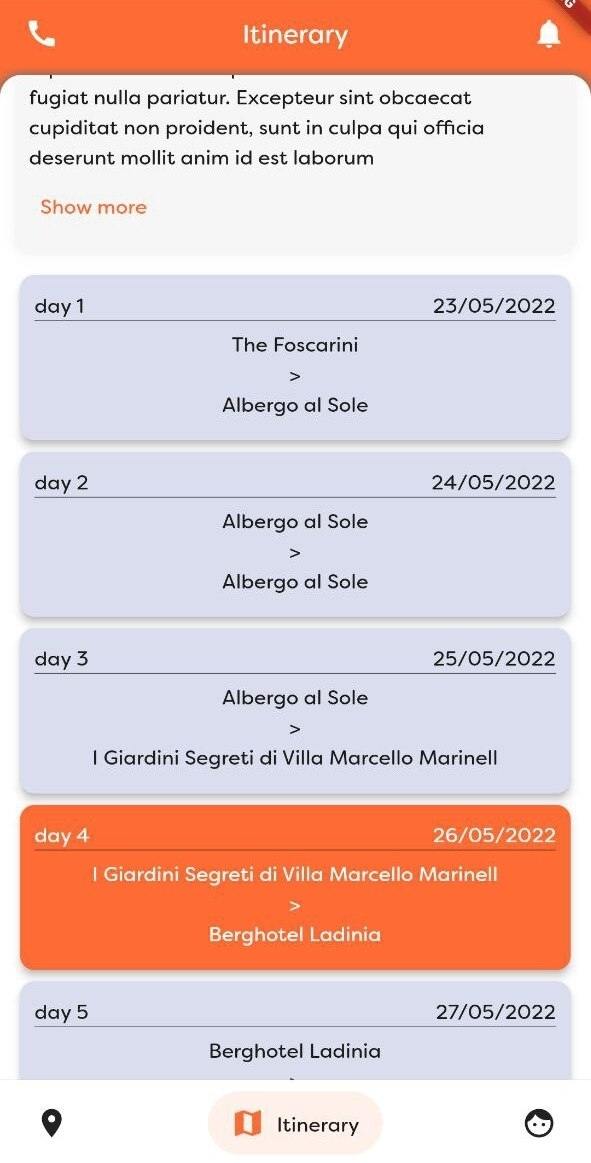
\includegraphics[width=0.3\columnwidth]{img/ch/itinerario.jpg}}
    \frame{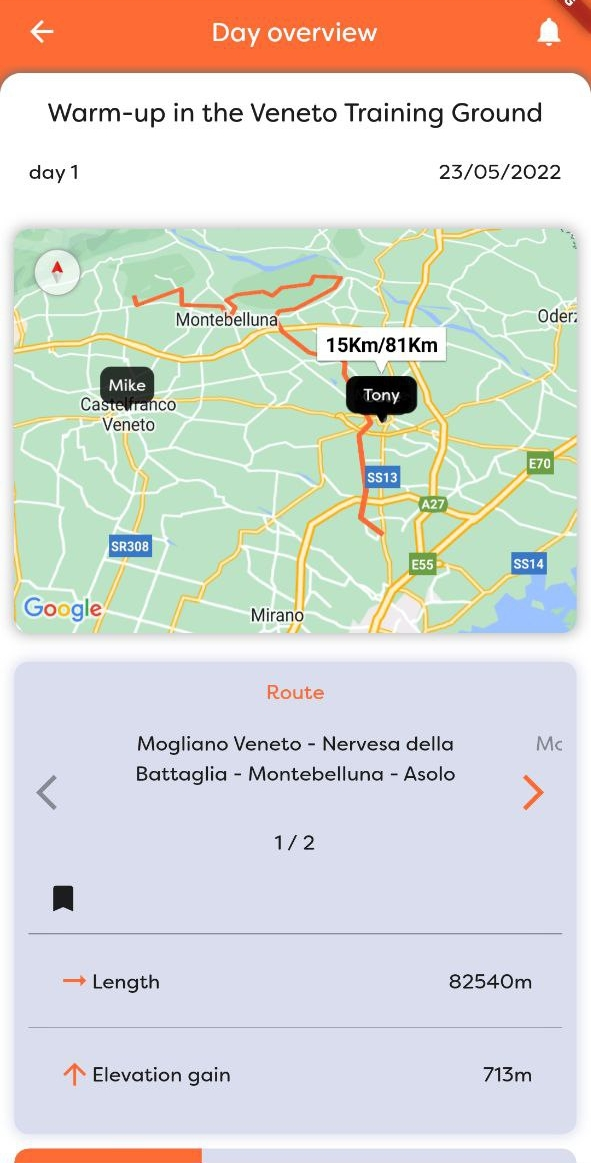
\includegraphics[width=0.3\columnwidth]{img/ch/route.jpg}}
    \frame{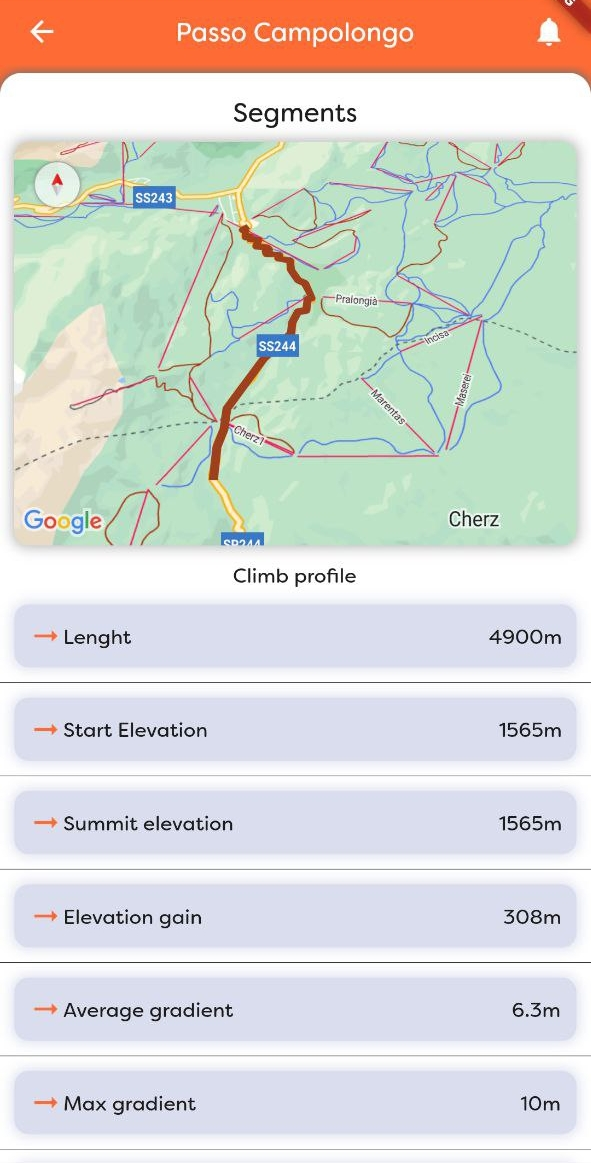
\includegraphics[width=0.3\columnwidth]{img/ch/climb.jpg}}
    \caption{Da sinistra verso destra: schermata delle giornate di un \textit{tour}, schermata di una giornata in dettaglio, schermata di un \textit{climb} in dettaglio.}
    \label{fig:inter-route}
\end{figure}

\subsubsection{Implementazione}
La schermata di una giornata in dettaglio è basata fondamentalmente sulle seguenti classi:
\begin{itemize}
    \item \textbf{DayScreen}: determina l'aspetto grafico della schermata, qui viene definita la gerarchia di \textit{widget} che compone la schermata. Visualizza una mappa della \textit{route} selezionata, un carosello per modificare la selezione, un carosello per visualizzare i \textit{POI} della \textit{route} e altre informazioni minori sulla giornata. I principali \textit{widget} utilizzati sono: \textit{GoogleMapCh} per: visualizzare la mappa, disegnare gli utenti, disegnare la \textit{route} percorsa, disegnare i \textit{climb} e \textit{Swiper} creare i caroselli;
    \item \textbf{DayBloc}: rappresenta l'aspetto logico della schermata e svolge tre importanti compiti:
    \begin{itemize}
        \item definisce tutti gli eventi inerenti alla schermata, tra cui \textit{SwitchRouteEvent} e \textit{SwitchClimbEvent} per selezionare rispettivamente una nuova \textit{route} e un nuovo \textit{climb};
        \item definisce lo stato della schermata, mantiene la \textit{route} selezionata, \textit{climb} selezionato e i relativi \gls{gpxg};
        \item gestisce gli eventi in arrivo interfacciandosi con lo strato sottostante, con il \textit{RouteRepository} e il \textit{ClimbRepository} per l'ottenimento dei \textit{GPX}.
    \end{itemize}
    \item \textbf{RouteSqlDao}: è una classe da me concepita implementare il salvataggio in locale dei \textit{GPX}, evitando quindi di dover richiedere al \textit{back-end} dati già ricevuti.
\end{itemize}

\begin{figure}[!h]
    \centering
    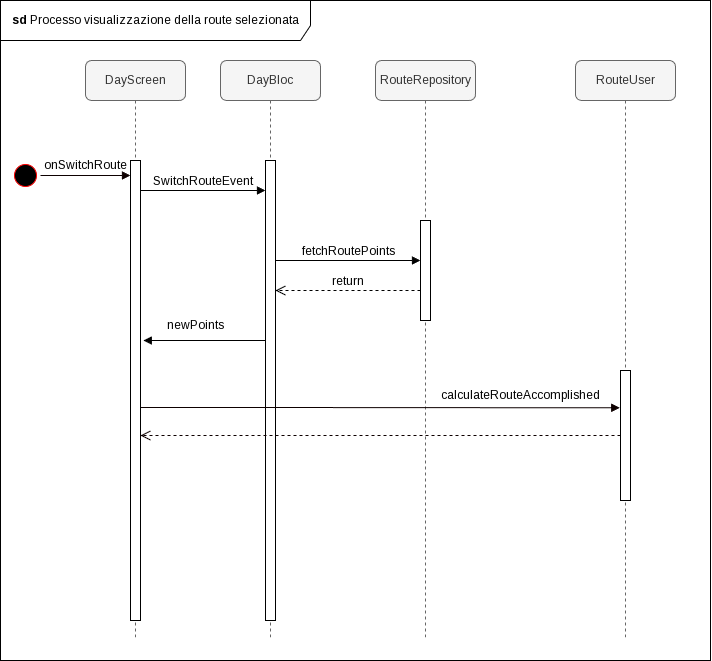
\includegraphics[width=0.9\columnwidth]{img/codifica/seq-route.png}
    \caption{Diagramma di sequenza per il processo di calcolo della \textit{route percorsa}.}
    \label{fig:seq-route}
\end{figure}

\noindent Il diagramma di sequenza in figura \ref{fig:seq-route} mostra il normale processo di selezione di una nuova \textit{route} visualizzata: per prima cosa \textit{DayBloc} richiede al \textit{RouteRepository} i dati necessari, a quel punto il \textit{repository} applica una semplice politica di selezione, restituisce il \textit{GPX} in locale nel caso sia stato ricevuto in precedenza, altrimenti esegue una nuova richiesta al \textit{RouteHttpDao} per ottenere i dati e salvarli in locale. Dopo aver ricevuto i dati, \textit{DayBloc} li fornisce al \textit{DayScreen}, il quale tramite la posizione dell'utente corrente esegue il calcolo della \textit{route} percorsa. 

\paragraph{Algoritmo di calcolo della \textit{route} percorsa}
Il calcolo della \textit{route} percorsa è un semplice algoritmo che data una posizione e un insieme di punti geografici, esegue una ricerca per identificare il punto di minor distanza dalla posizione interessata. Dal punto ottenuto viene calcolata la distanza totale percorsa sommando cumulativamente le distanze dei punti precedenti\footcite{site:gpx-doc}. 

\subsubsection{Resoconto dei requisiti associati}
La tabella \ref{tab:req-tour-stato} elenca i requisiti associati alla gestione dell'itinerario. Ogni requisito identificato è stato soddisfatto e validato dal cliente.

\begin{longtable}{ |p{2cm}|p{8cm}|p{2cm}|  }
    \caption{Soddisfacimento dei requisiti associati alla gestione dell'itinerario.}
    \label{tab:req-tour-stato}
    \hline
    \textbf{Codice} & \textbf{Descrizione} & \textbf{Stato}
    \hline
    \textbf{ROF9}   & L'utente autenticato deve poter visualizzare la mappa dell'itinerario. & \textbf{Soddisfatto}   \\ \hline
    \textbf{ROF9.1} & L'utente autenticato deve poter visualizzare la sua distanza con gli altri partecipanti. & \textbf{Soddisfatto} \\ \hline
    \textbf{ROF9.2} & L'utente autenticato deve poter visualizzare l'accuratezza del suo segnale \textit{GPS}. & \textbf{Soddisfatto} \\ \hline
    \textbf{ROF10}  & L'utente autenticato deve poter ricentrare la mappa nella sua posizione. & \textbf{Soddisfatto}  \\ \hline
    \textbf{ROF11}  & L'utente autenticato deve modificare lo stato di condivisione della propria posizione. & \textbf{Soddisfatto}  \\ \hline
    \textbf{ROF11.1} & L'utente autenticato deve poter attivare la condivisione della posizione. & \textbf{Soddisfatto} \\ \hline
    \textbf{ROF11.2} & l'utente autenticato deve poter disattivare la condivisione della posizione. & \textbf{Soddisfatto} \\ \hline
    \textbf{ROF12} & Il tentativo di attivazione della condivisione della posizione deve fallire nel caso in cui il GPS non sia attivo. & \textbf{Soddisfatto} \\ \hline
    \textbf{ROF13} & L'utente autenticato deve poter visualizzare tutte le giornate dell'itinerario corrente. & \textbf{Soddisfatto} \\ \hline
    \textbf{ROF14} & L'utente autenticato deve poter visualizzare una giornata nel dettaglio. & \textbf{Soddisfatto4} \\ \hline
    \textbf{ROF14.1} & L'utente autenticato deve poter visualizzare la mappa durante l'attività di visualizzazione di una giornata nel dettaglio. & \textbf{Soddisfatto} \\ \hline
    \textbf{ROF14.1.1} & L'utente autenticato deve poter visualizzare i partecipanti durante l'attività di visualizzazione della mappa di una giornata. & \textbf{Soddisfatto}\\ \hline
    \textbf{ROF14.1.2} & L'utente autenticato deve poter visualizzare tutti i \textit{POI} durante l'attività di visualizzazione della mappa di una giornata. & \textbf{Soddisfatto}\\ \hline
    \textbf{ROF14.1.3} & L'utente autenticato deve poter visualizzare la \textit{route} percorsa di un partecipante durante l'attività di visualizzazione della mappa di una giornata. & \textbf{Soddisfatto}\\ \hline
    \textbf{ROF14.1.4} & L'utente autenticato deve poter visualizzare la \textit{route} selezionata durante l'attività di visualizzazione della mappa di una giornata. & \textbf{Soddisfatto} \\ \hline
    \textbf{ROF14.1.5} & L'utente autenticato deve poter visualizzare il \textit{climb} selezionato durante l'attività di visualizzazione della mappa di una giornata. & \textbf{Soddisfatto} \\ \hline
    \textbf{ROF14.1.6} & I \textit{POI} generici e speciali devono essere visualizzati differentemente nella mappa di una giornata. & \textbf{Soddisfatto} \\ \hline
    \textbf{ROF14.2} & L'utente autenticato deve poter visualizzare i \textit{climb} di una giornata durante l'attività di visualizzazione di una giornata nel dettaglio. & \textbf{Soddisfatto} \\ \hline
    \textbf{ROF14.3} & L'utente autenticato deve poter visualizzare i \textit{poi} di una giornata durante l'attività di visualizzazione di una giornata nel dettaglio. & \textbf{Soddisfatto} \\ \hline
    \textbf{ROF15} & L'utente autenticato deve poter modificare la \textit{route} selezionata in una giornata. & \textbf{Soddisfatto} \\ \hline
    \textbf{ROF16} & L'utente autenticato deve poter modificare il \textit{climb} selezionato in una giornata. & \textbf{Soddisfatto} \\ \hline
    \textbf{ROV3} & La giornata corrente di un itinerario deve essere evidenziata. & \textbf{Soddisfatto} \\ \hline
    \textbf{RDV5} & Il tratto di \textit{route} percorsa deve essere visualizzata nella mappa. & \textbf{Soddisfatto} \\ \hline
    \textbf{ROV6} & I \textit{POI} normali devono essere visulizzati differentemente da quelli speciali. & \textbf{Soddisfatto} \\ \hline
    \textbf{RDP3} & I \textit{GPX} non devono essere richiesti più di una volta & \textbf{Soddisfatto} \\ \hline
\end{longtable}

\newpage
\section{Verifica e validazione}
In questa sezione viene descritto i processi di verifica e validazione attuati durante il progetto. Con verifica si intendono tutte le pratiche adottate al fine di prevenire l'introduzione di errori all'interno del prodotto, mentre con validazione si intende il processo di accertamento dei requisiti. Per quanto riguarda la verifica, per i \textit{test} statici mi sono avvalso del \gls{linterg} ufficiale di \textit{Flutter}, il quale va a eseguire un'analisi statica del codice seguendo determinate regole preconfigurate\footcite{site:linter-doc}, ciò mi ha permesso di applicare uno stile di codifica consistente in tutto il progetto ed evitare eventuali errori sintattici. I \textit{test} dinamici sono stati fatti manualmente da me con l'aiuto del \gls{debuggerg} di \textit{VSCode}, non sono riuscito a creare una \textit{suit} di \textit{testing} per automatizzare la verifica in quanto le brevi tempistiche di rilascio non mi hanno permesso di concentrarmi in attività secondarie allo sviluppo.
Per quanto riguarda la validazione, questa è stata perseguita periodicamente insieme al \textit{project manager} prima di ogni rilascio, verificando il soddisfacimento degli obiettivi prefissati nel \textit{sprint planning}. 
